\documentclass[12pt]{report} %fuente a 12pt

% MÁRGENES: 2,5 cm sup. e inf.; 3 cm izdo. y dcho.
\usepackage[
a4paper,
vmargin=2.5cm,
hmargin=3cm
]{geometry}

% INTERLINEADO: Estrecho (6 ptos./interlineado 1,15) o Moderado (6 ptos./interlineado 1,5)
\renewcommand{\baselinestretch}{1.15}
\parskip=6pt

% DEFINICIÓN DE COLORES para portada y listados de código
\usepackage[table]{xcolor}
\definecolor{azulUC3M}{RGB}{0,0,102}
\definecolor{gray97}{gray}{.97}
\definecolor{gray75}{gray}{.75}
\definecolor{gray45}{gray}{.45}

% Soporte para GENERAR PDF/A
\usepackage[a-1b]{pdfx}

% ENLACES
\usepackage{hyperref}
\hypersetup{colorlinks=true,
	linkcolor=black, % enlaces a partes del documento (p.e. índice) en color negro
	urlcolor=blue} % enlaces a recursos fuera del documento en azul

\usepackage{pdfpages}
\setlength{\parindent}{0em}

% EXPRESIONES MATEMATICAS
\usepackage{amsmath,amssymb,amsfonts,amsthm}

\usepackage{txfonts} 
\usepackage[T1]{fontenc}
\usepackage[utf8]{inputenc}

\usepackage{tikz}
\usepackage{pgfplots}

\usepackage[spanish, es-tabla]{babel} 
\usepackage[babel, spanish=spanish]{csquotes}
\AtBeginEnvironment{quote}{\small}

% diseño de PIE DE PÁGINA
\usepackage{fancyhdr}
\pagestyle{fancy}
\fancyhf{}
\renewcommand{\headrulewidth}{0pt}
\rfoot{\thepage}
\fancypagestyle{plain}{\pagestyle{fancy}}

% DISEÑO DE LOS TÍTULOS de las partes del trabajo (capítulos y epígrafes o subcapítulos)
\usepackage{titlesec}
\usepackage{titletoc}
\titleformat{\chapter}[block]
{\large\bfseries\filcenter}
{\thechapter.}
{5pt}
{\MakeUppercase}
{}
\titlespacing{\chapter}{0pt}{0pt}{*3}
\titlecontents{chapter}
[0pt]                                               
{}
{\contentsmargin{0pt}\thecontentslabel.\enspace\uppercase}
{\contentsmargin{0pt}\uppercase}                        
{\titlerule*[.7pc]{.}\contentspage}                 

\titleformat{\section}
{\bfseries}
{\thesection.}
{5pt}
{}
\titlecontents{section}
[5pt]                                               
{}
{\contentsmargin{0pt}\thecontentslabel.\enspace}
{\contentsmargin{0pt}}
{\titlerule*[.7pc]{.}\contentspage}

\titleformat{\subsection}
{\normalsize\bfseries}
{\thesubsection.}
{5pt}
{}
\titlecontents{subsection}
[10pt]                                               
{}
{\contentsmargin{0pt}                          
	\thecontentslabel.\enspace}
{\contentsmargin{0pt}}                        
{\titlerule*[.7pc]{.}\contentspage}  


% DISEÑO DE TABLAS.
\usepackage{multirow} % permite combinar celdas 
\usepackage{caption} % para personalizar el título de tablas y figuras
\usepackage{floatrow} % utilizamos este paquete y sus macros \ttabbox y \ffigbox para alinear los nombres de tablas y figuras de acuerdo con el estilo definido. Para su uso ver archivo de ejemplo 
\usepackage{array} % con este paquete podemos definir en la siguiente línea un nuevo tipo de columna para tablas: ancho personalizado y contenido centrado
\newcolumntype{P}[1]{>{\centering\arraybackslash}p{#1}}
\DeclareCaptionFormat{upper}{#1#2\uppercase{#3}\par}

% Diseño de tabla para ingeniería
\captionsetup[table]{
	format=upper,
	name=TABLA,
	justification=centering,
	labelsep=period,
	width=.75\linewidth,
	labelfont=small,
	font=small,
}

% DISEÑO DE FIGURAS.
\usepackage{graphicx}
\graphicspath{{img/}} %ruta a la carpeta de imágenes

% Diseño de figuras para ingeniería
\captionsetup[figure]{
	format=hang,
	name=Fig.,
	singlelinecheck=off,
	labelsep=period,
	labelfont=small,
	font=small		
}

% NOTAS A PIE DE PÁGINA
\usepackage{chngcntr} %para numeración contínua de las notas al pie
\counterwithout{footnote}{chapter}

% LISTADOS DE CÓDIGO
% soporte y estilo para listados de código. Más información en https://es.wikibooks.org/wiki/Manual_de_LaTeX/Listados_de_código/Listados_con_listings
\usepackage{listings}

% definimos un estilo de listings
\lstdefinestyle{estilo}{ frame=Ltb,
	framerule=0pt,
	aboveskip=0.5cm,
	framextopmargin=3pt,
	framexbottommargin=3pt,
	framexleftmargin=0.4cm,
	framesep=0pt,
	rulesep=.4pt,
	backgroundcolor=\color{gray97},
	rulesepcolor=\color{black},
	%
	basicstyle=\ttfamily\footnotesize,
	keywordstyle=\bfseries,
	stringstyle=\ttfamily,
	showstringspaces = false,
	commentstyle=\color{gray45},     
	%
	numbers=left,
	numbersep=15pt,
	numberstyle=\tiny,
	numberfirstline = false,
	breaklines=true,
	xleftmargin=\parindent
}

\captionsetup[lstlisting]{font=small, labelsep=period}
% fijamos el estilo a utilizar 
\lstset{style=estilo}
\renewcommand{\lstlistingname}{\uppercase{Código}}

\pgfplotsset{compat=1.17} 
%-------------
%	DOCUMENTO
%-------------

\begin{document}
\pagenumbering{roman} % Se utilizan cifras romanas en la numeración de las páginas previas al cuerpo del trabajo
	
%----------
%	PORTADA
%----------	
\begin{titlepage}
	\begin{sffamily}
	\color{azulUC3M}
	\begin{center}
		\begin{figure}[H] %incluimos el logotipo de la Universidad
			\makebox[\textwidth][c]{
\includegraphics[width=16cm]{Portada_Logo.png}}
		\end{figure}
		\vspace{2.5cm}
		\begin{Large}
			Grado en Ingeniería Informática\\			
			2020-2021\\
			\vspace{2cm}		
			\textsl{Apuntes}\\
			\bigskip
		\end{Large}
		 	{\Huge Procesadores de Lenguaje}\\
		 	\vspace*{0.5cm}
	 		\rule{10.5cm}{0.1mm}\\
			\vspace*{0.9cm}
			{\LARGE Jorge Rodríguez Fraile\footnote{\href{mailto:100405951@alumnos.uc3m.es}{Universidad: 100405951@alumnos.uc3m.es}  |  \href{mailto:jrf1616@gmail.com}{Personal: jrf1616@gmail.com}}}\\ 
			\vspace*{1cm}
	\end{center}
	\vfill
	\color{black}
		
\includegraphics[width=4.2cm]{img/creativecommons.png}\\
		Esta obra se encuentra sujeta a la licencia Creative Commons\\ \textbf{Reconocimiento - No Comercial - Sin Obra Derivada}
	\end{sffamily}
\end{titlepage}

%----------
%	ÍNDICES
%----------	

%--
% Índice general
%-
\tableofcontents
\thispagestyle{fancy}

%--
% Índice de figuras. Si no se incluyen, comenta las líneas siguientes
%-
\listoffigures
\thispagestyle{fancy}

%--
% Índice de tablas. Si no se incluyen, comenta las líneas siguientes
%-
\listoftables
\thispagestyle{fancy}

%----------
%	TRABAJO
%----------	
\clearpage
\pagenumbering{arabic} % numeración con números arábigos para el resto de la publicación	


%----------
%	COMENZAR A ESCRIBIR AQUI
%----------	

\section{Información}

\begin{quote}
Teorías: Antonio Berlanga de Jesús y Jesús García Herrero

Prácticas: Juan Manuel Alonso Weber jmaw@ia.uc3m.es
\end{quote}

\section{Presentación}

Practicas semanales de 2 en 2.

Hay clases en el cronograma de más, algunas se usarán para recuperar.

Las practicas las hacemos en Linux, vale, máquina virtual, guernika y se
puede hacer en WSL2. Lo importante es tener un terminal.

Vamos a usar bison y flex, programaremos en C. El editor de texto que
queramos.

\chapter{Repaso de TALF}

\section{Definiciones}

\textbf{Forma sentencial}: Aplicando reglas de producción llego a
\(x \in \sum^*\)

\textbf{Sentencia}: Forma sentencial en el que x no tiene No Terminales.

\textbf{Lenguaje asociado a una gramática}: Todas las sentencias, sin
terminales, de una gramática.

\textbf{Recursividad}: Aparece el terminal de la parte izquierda a la
derecha.

\begin{itemize}
\item
  Recursividad a izquierda: $A \rightarrow Ay$
\item
  Recursividad a derechas: $A \rightarrow xA$
\end{itemize}

\textbf{Reglas compresoras}: Aquellas que producen menos símbolos de los
que hay a la izquierda. Como lo es \(x::= \lambda\)

\section{Gramática}

\(G=\{ \sum_T, \sum_N, S, P\}\)

\begin{itemize}
\item
  \(\sum_T\): Conjunto de símbolos \textbf{terminales}, alfabeto del
  lenguaje.
\item
  \(\sum_N\): Conjunto de símbolos \textbf{no terminales}.
\item
  \(S\): \textbf{Axioma} \(S \in \sum_N\)
\item
  \(P\): Conjunto de \textbf{Reglas de producción}.
\item
  Backus Normal Form: \(P_i ::= P_d\)
\item
  \(P_i \in (\sum_T \cup \sum_N)^+\) Al menos un símbolo
\item
  \(P_d \in (\sum_T \cup \sum_N)^*\) De 0 a infinitos símbolos
\item
  \(\lambda\) Clausula vacía
\end{itemize}


\subsection{Tipos de Gramáticas}

\textbf{Tipo 3}: Autómata Finito Determinista y Autómata Finito No
Determinista.

\begin{itemize}
\item
  Expresiones regulares o lineales.
\item
  Un solo No Terminal para dar:
  \(P_d ::= a | aN | Na; a \in \sum_T, N \in \sum_N\)
\item
  Lineal izquierda: \(P_d ::= a | Na\)
\item
  Lineal derecha: \(P_d ::= a | aN\)
\end{itemize}

\textbf{Tipo 2}: Autómata a Pila.

\begin{itemize}
\item
  Lenguaje Independiente del Contexto.
\item
  Un No Terminal para dar cualquier sentencia, excepto lambda que solo
  lo puede dar el axioma.
\end{itemize}

\textbf{Tipo 1}: Maquina Linealmente Acotada.

\begin{itemize}
\item
  Lenguaje de contexto libre.
\item
  Cualquier sentencia para dar cualquier secuencia, pero que no sea una
  regla reductora(tampoco se puede No Terminal para dar lambda).
\end{itemize}

\textbf{Tipo 0}: Maquina de Turing.

\begin{itemize}
\item
  Lenguaje sin restricciones.
\item
  Cualquier sentencia para dar cualquier secuencia de símbolos, incluso
  reglas reductoras.
\end{itemize}

\section{Problemas de lectura de sentencias}

\textbf{Precedencia}: Hay operadores con mayor prioridad. Se debe hacer
desde lo último derivado hacia arriba. Esto provoca ambigüedad, que es
nuestro enemigo.

\begin{figure}[H]
	\ffigbox[\FBwidth]
	{\caption{Ejemplo Precedencia}}
	{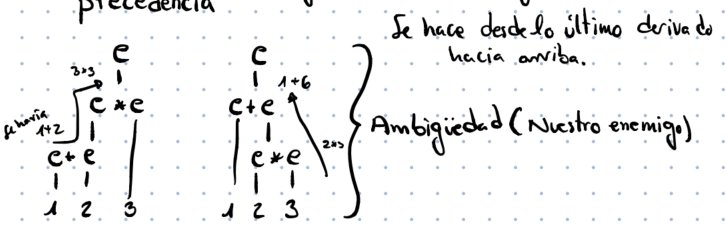
\includegraphics[scale=.4]{Untitled.png}}
\end{figure}

\textbf{Dangling Else}: Sobre a quién pertenece el else, en C el else
pertenece al último else.

\begin{lstlisting}[language=C]
if C1 then A else if C2
then B else C
\end{lstlisting}

\textbf{Asociatividad}: Entre operaciones con la misma precedencia.
1-1-1-1


\section{Derivación}

Aplicación de una producción a una forma sentencial.

\textbf{Derivación más a la izquierda}: Sustituye el símbolo no terminal
más a la izquierda.

\textbf{Derivación más a la derecha}: Sustituye el símbolo no terminal
más a la derecha.


\section{Ambigüedad}

Hay distintos niveles:

\begin{itemize}

\item
  \textbf{Sentencia}: Se puede obtener por dos derivaciones diferentes.
\item
  \textbf{Gramática}: Si puede obtener una sentencia con dos
  derivaciones.
\item
  \textbf{Lenguaje}: Todas las gramáticas que lo generan son ambiguas
  entonces es inherentemente ambiguo.
\end{itemize}


\section{Bien formar Gramáticas}

\textbf{Limpiar}:

\begin{enumerate}
\def\labelenumi{\arabic{enumi}.}
\item
  Sin \textbf{reglas innecesarias}: Un terminal que se da a sí mismo.
  A→A
\item
  Sin \textbf{símbolos inaccesibles}: Poner T y NT, e ir tachando según
  aparecen, los que no aparecen regla fuera.
\item
  Sin \textbf{símbolos superfluos}: Empezamos con las reglas que solo
  producen terminales e ir subiendo por pasos.
\end{enumerate}

Sin reglas \textbf{no generativas}: Las que dan lambda, quitarlas y
sustituir sus apariciones por lambda(nada).

Sin reglas de \textbf{redenominación}: Las que llaman aun solo símbolo
No Terminal, poner las reglas de ese símbolo en el que lo invoca.


\section{Transformaciones útiles en compiladores}

Estas transformaciones facilitan a los analizadores predictivos. Estos
analizadores implican que nunca se va a hacer backtracking siempre
sabemos que regla de producción hay que aplicar o no hay más, pero no se
retrocede.

\textbf{Factorización a izquierdas}

\begin{itemize}
\item
  Cuando hay una estructura común en las reglas de producción.
\item
  Se crea un nuevo No terminal para dar los símbolos que acompañan a esa
  parte común, en el original se pone la parte común seguida del nuevo
  símbolo.
\end{itemize}

\begin{figure}[H]
	\ffigbox[\FBwidth]
	{\caption{Algoritmo de Factorización a Izquierdas}}
	{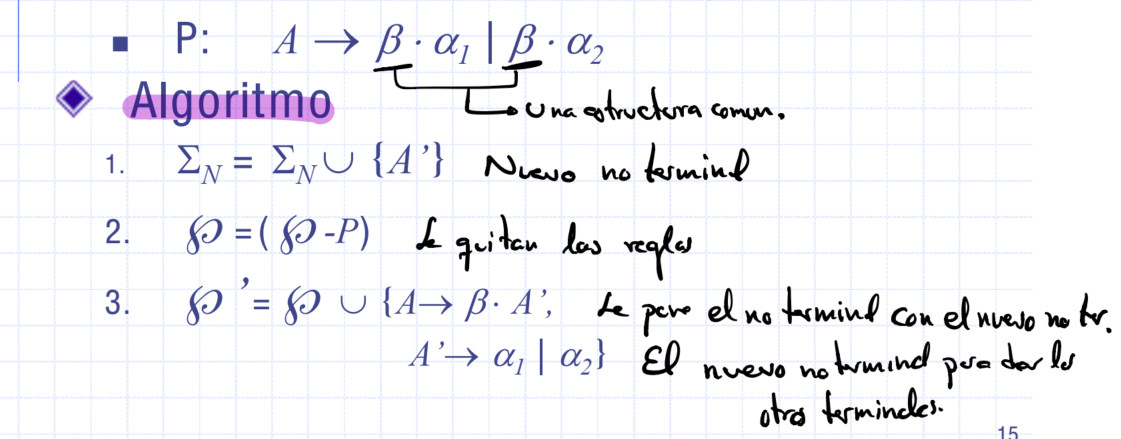
\includegraphics[scale=.3]{Untitled 1.png}}
\end{figure}

\textbf{Eliminar recursividad por la izquierda}

\begin{itemize}
\item
  Para evitar recursividades pendientes, ya que leemos de izquierda a
  derecha, así reconocemos mientras aplicamos reglas.
\item
  A las reglas no recursivas a izquierda se le concatena un nuevo No
  Terminal (quitamos las que eran recursivas).
\item
  Ese nuevo símbolo produce \(\lambda\) y lo que producía originalmente
  que era recursivo a izquierda, pero en recursividad a la derecha.
\end{itemize}

\begin{figure}[H]
	\ffigbox[\FBwidth]
	{\caption{Algoritmo de Eliminación de recursividad a Izquierdas}}
	{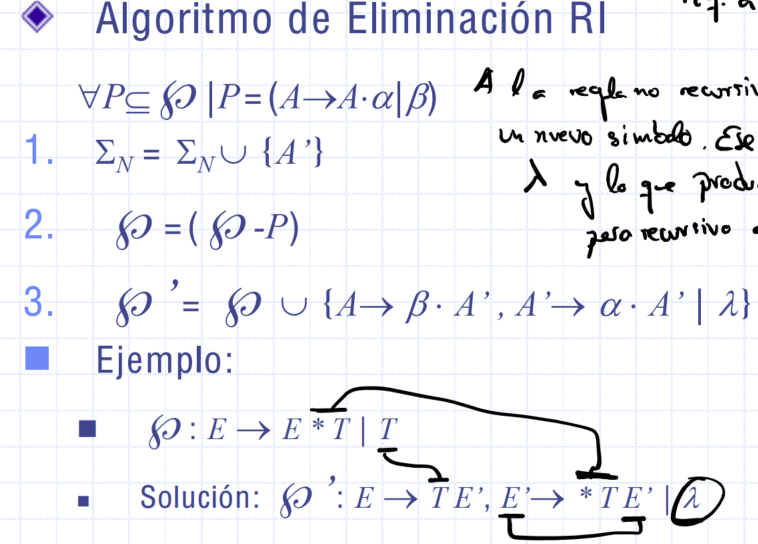
\includegraphics[scale=.4]{Untitled 2.png}}
\end{figure}

\section{Autómata Finito Determinista}

\(AFD=( \sum, Q, f, q_o, F)\)

\textbf{Donde:}

\begin{itemize}
\item
  \(\sum\) Símbolos de entrada, Tokens.
\item
  \(Q\) Estados.
\item
  \(q_o \in Q\) Estado inicial.
\item
  \(F \subseteq Q\) Estados finales.
\item
  \(f(q,a \cdot x)\) Función de transición. Con un estado y un símbolo,
  voy a un estado.
\end{itemize}

\begin{figure}[H]
	\ffigbox[\FBwidth]
	{\caption{Diagrama AFD}}
	{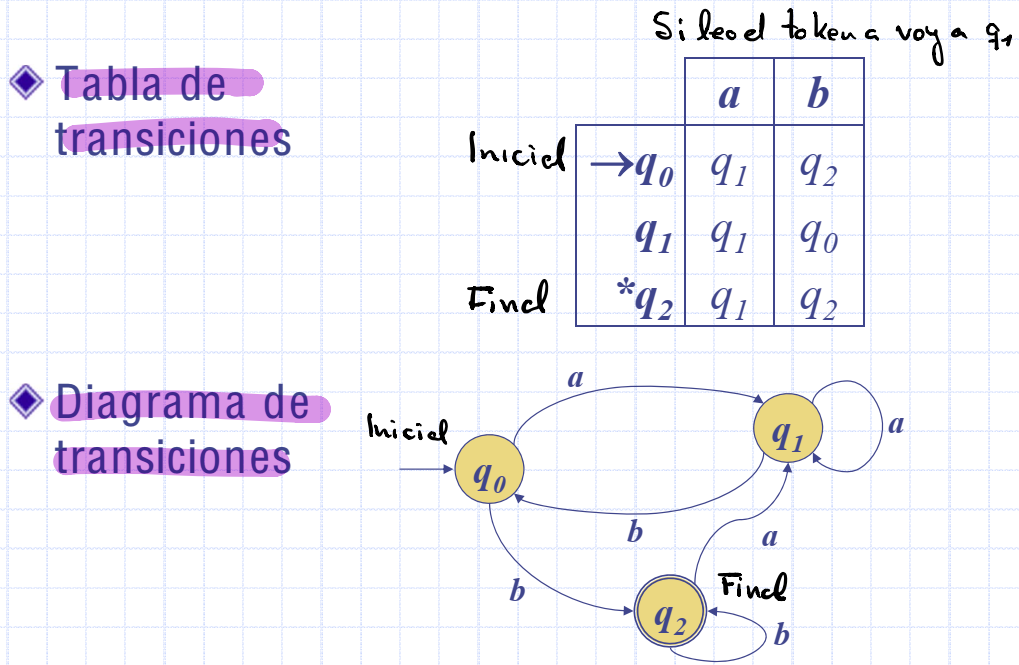
\includegraphics[scale=.25]{Untitled 3.png}}
\end{figure}

Extensión a palabras: Recibe una palabra y va cogiendo los símbolos de
entrada, y aplicando reglas sucesivas. Palabras que partiendo del
inicial nos permite llegar a uno final.

\textbf{Lenguaje asociado:} Aquellas palabras tales que aplicando
extensión a palabra el \(q_o\) alcanza su estado de F, final.

\textbf{Equivalencia de AFD:} Si el lenguaje que reconocen es el mismo.

\textbf{Minimización de AFD:} Autómata finito mínimo equivalente es
aquel con menor número de estado, pero mismo lenguaje.

Siempre se puede pasar de G3 a AFD, aunque puede que no directo, por
medio de AFND.


\section{Autómata Finito No Determinista}

\begin{itemize}
\item
  Admite \(\lambda\) y más de una posibilidad por símbolo.
\item
  \(AFND=( \sum, Q, f, q_o, F)\) Los símbolos representan lo mismo que
  en AFD.
\item
  En este caso se permite transicionar sin recibir símbolo, lambda,
  además, varias transiciones para un mismo símbolo en un mismo estado.
\end{itemize}

\begin{figure}[H]
	\ffigbox[\FBwidth]
	{\caption{Diagrama AFND}}
	{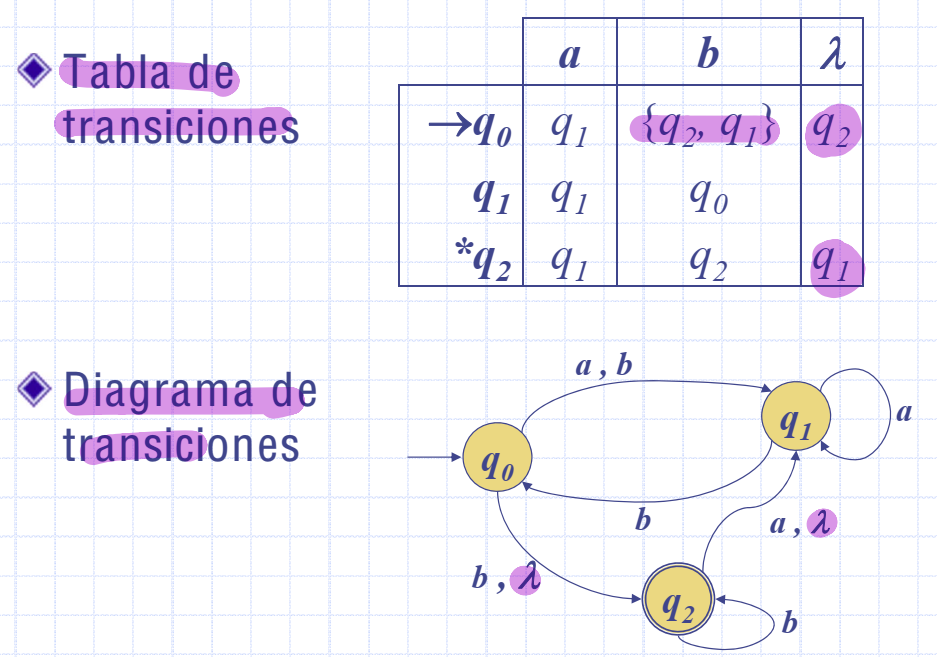
\includegraphics[scale=.4]{Untitled 4.png}}
\end{figure}

Para cualquier AFD existe uno no determinista equivalente.

Para toda gramática G3 existe un autómata determinista y no
determinista.


\section{Autómata a Pila (G2)}

\(AP=(\sum, \Gamma, Q, A_0, q_0, f, F)\)

\textbf{Donde:}

\begin{itemize}
\item
  \(\Gamma\) Conjunto de símbolos de pila
\item
  \(A_0\) Símbolo de pila inicial
\item
  \(f(q,\lambda,A)\) Transita a uno o varios estados y puede escribir o
  no en pila, cuando escribe pueden ser más de 1.
\item
  Para toda gramática G2 existe un AP.
\item
  El AP puede ser no determinista y en general
  \(APND \nrightarrow APD\).
\item
  Lenguaje aceptado por un AP, palabras que reconoce, y el final lo
  determina:
\end{itemize}

\textbf{Por estado final:} Cuando llega a un estado final y la secuencia
de entrada, está vacía, termina.

\textbf{Por vaciado de pila:} Entrada y pila vacía, termina.


\section{Expresiones Regulares G3}

\textbf{Definición:}

\begin{itemize}
\item
  \(\empty\) es una ER.
\item
  \(\lambda\) es una ER.
\item
  a es una ER, siendo a un Tokens.
\item
  \(\alpha + \beta\) es una ER, la unión.
\item
  \(\alpha \cdot \beta\) es una ER, la concatenación.
\item
  \(\alpha ^*\) es una ER, la clausura.
\end{itemize}

\textbf{ER útiles:}

\begin{itemize}
\item
  \(\alpha ^+ =\alpha \cdot \alpha ^*= \alpha ^* \cdot \alpha\) Al menos
  1
\item
  \(\alpha? = \alpha | \lambda\) Puede ser alpha o lambda
\item
  \([abc] = a|b|c\) Es a o b o c
\item
  \([a-z] = a|b|...|z\)
\end{itemize}

Dos EERR son equivalentes si describen el mismo lenguaje.

\begin{figure}[H]
	\ffigbox[\FBwidth]
	{\caption{Reglas de EERR}}
	{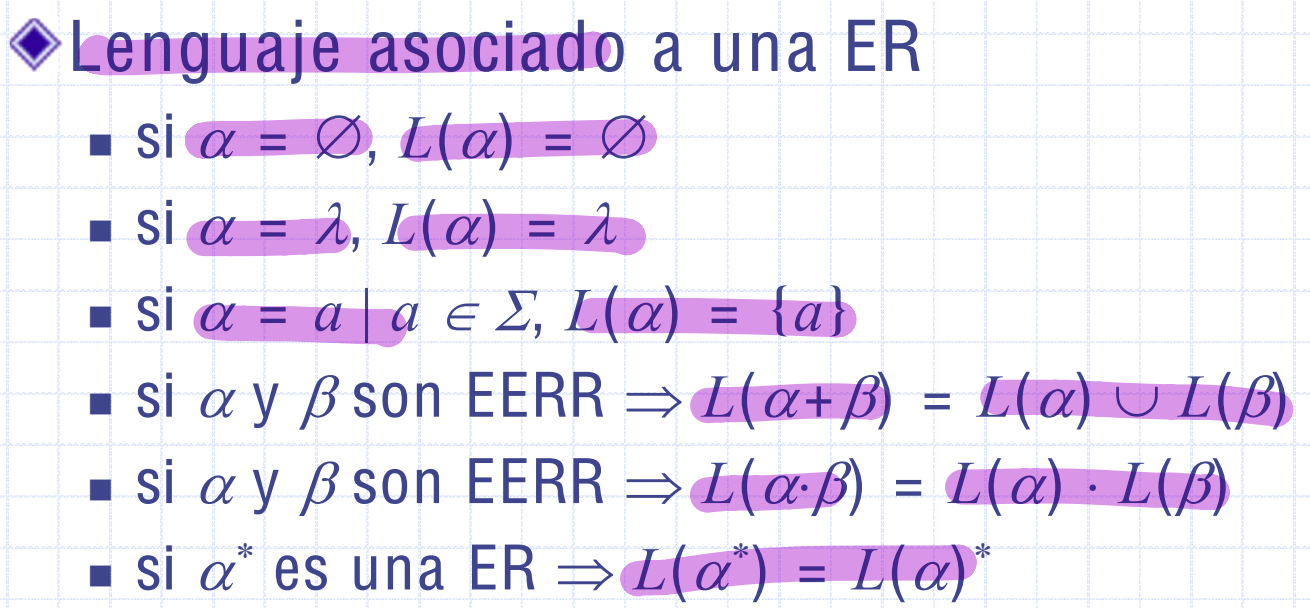
\includegraphics[scale=.15]{Untitled 5.png}
	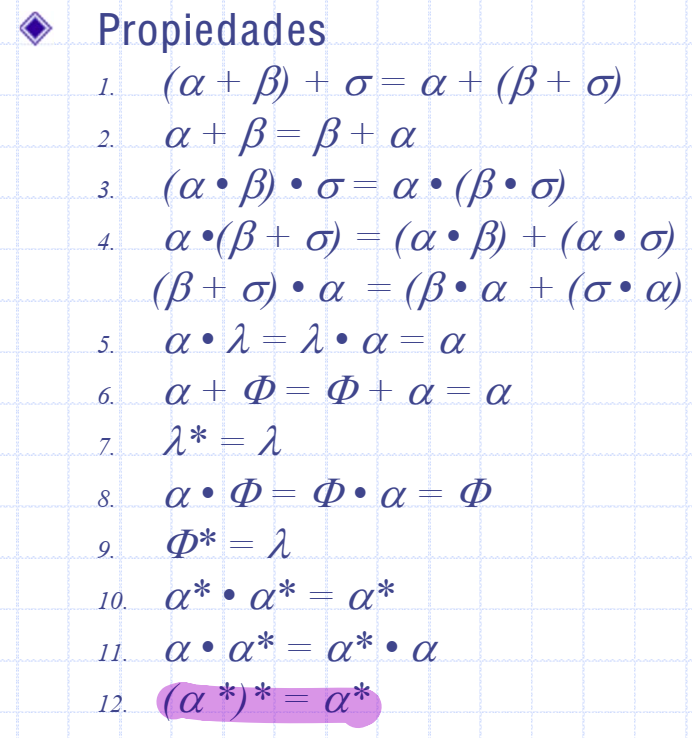
\includegraphics[scale=.25]{Untitled 6.png}}
	{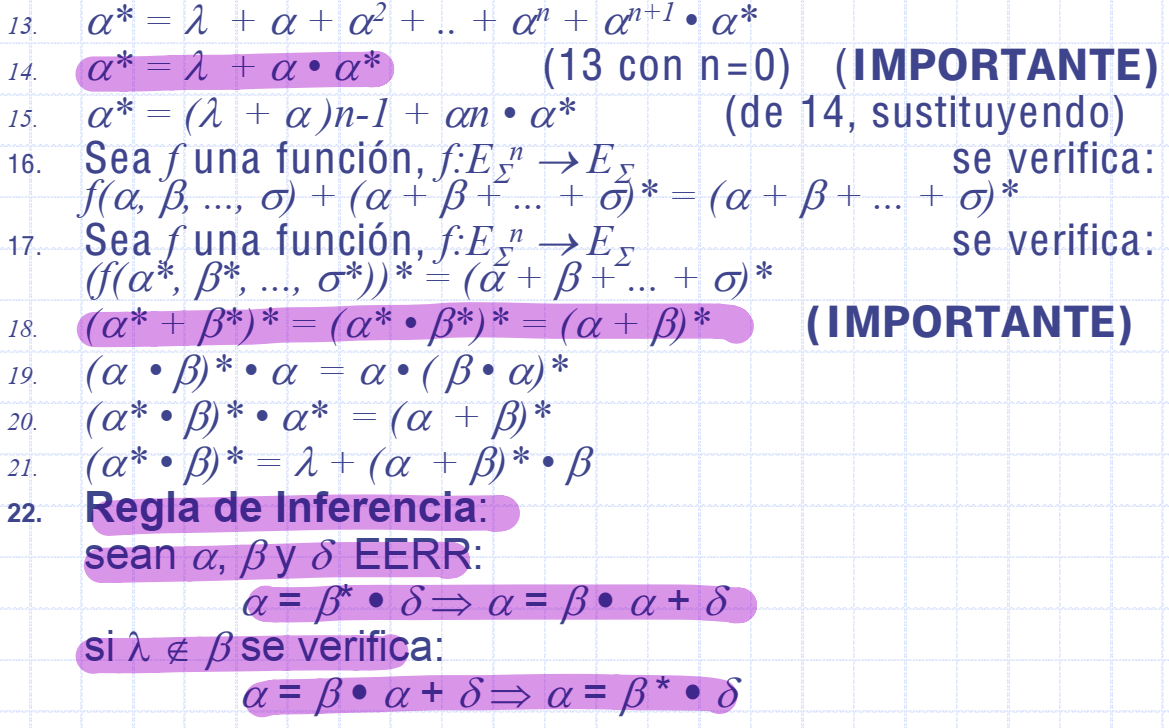
\includegraphics[scale=.3]{Untitled 7.png}}
\end{figure}

Inferencia: Si X=AX+B entonces X=A*B

\chapter{Tema 1: Introducción}

\textbf{Compilador}: Proceso de traducción que convierte un programa
fuente escrito en un lenguaje de alto nivel a un programa objeto en
código maquina y listo por tanto para ejecutarse en el ordenador. Solo
se genera el programa objeto cuando no hay errores.

\begin{figure}[H]
	\ffigbox[\FBwidth]
	{\caption{Diagrama tipos de programación}}
	{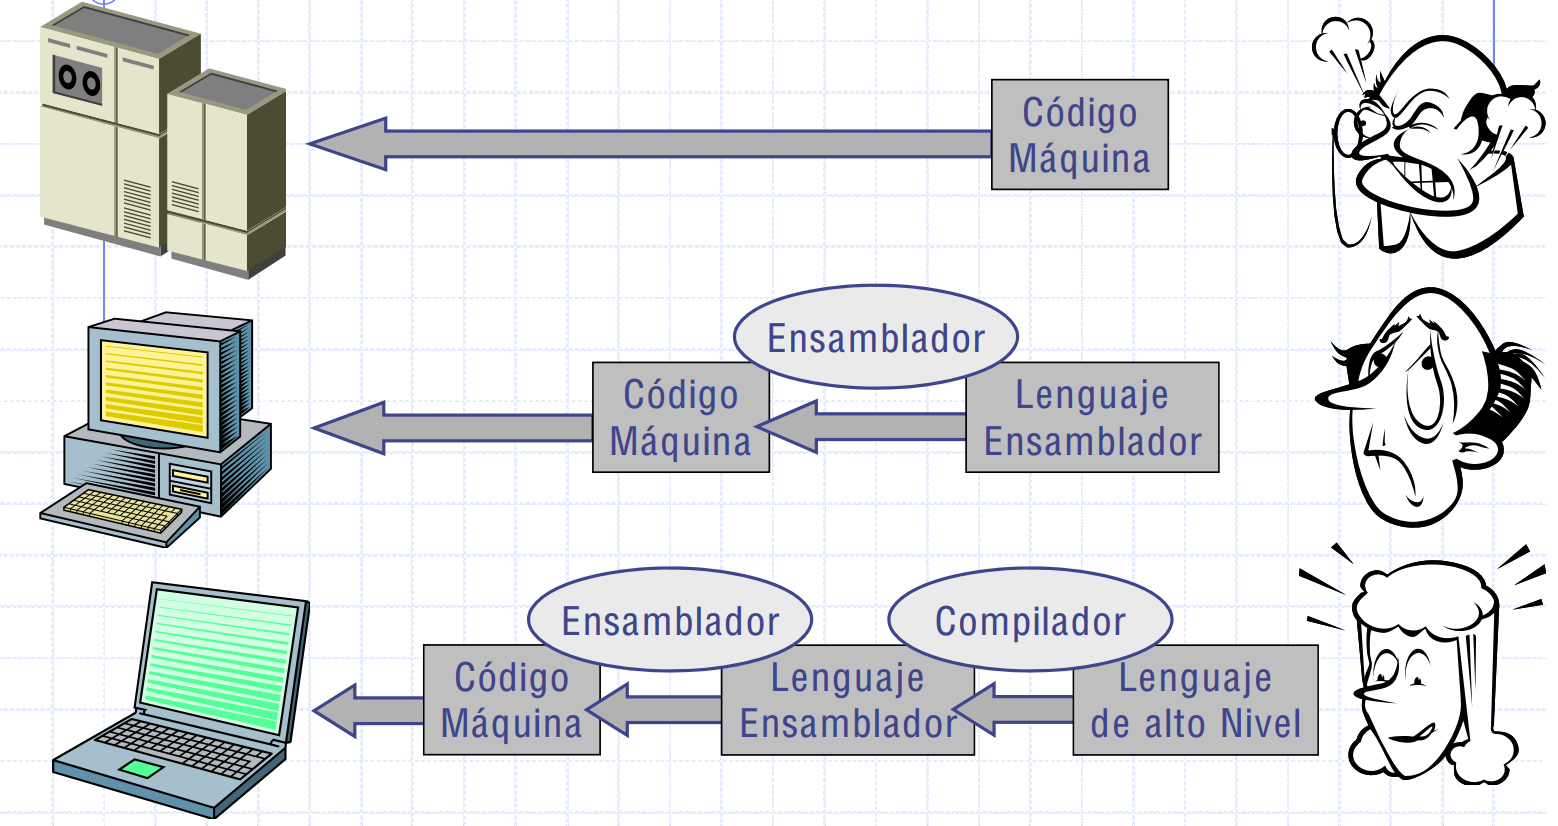
\includegraphics[scale=.25]{Untitled 8.png}}
\end{figure}

\textbf{Programa fuente → Compilador → Programa objeto/Mensajes de
error.}

Originalmente, cuando no existía se metía con 1's y 0's, código máquina.

Después, se creó el ensamblador que traduce un código nemotécnico
(lenguaje ensamblador) a código máquina.

Por último, el compilador sobre el ensamblador, esto facilito mucho las
cosas.

En los 50's se consideraban los programas más difíciles.

Con el tiempo se ha facilitado mucho con entornos de programación y
herramientas, no hay una fecha exacta del primer compilador.

Los primeros traducían formulas aritméticas a código máquina.

\textbf{Motivación}:

\begin{itemize}

\item
  Saber cómo se obtiene un ejecutable para alcanzar mejor eficiencia y
  corrección.
\item
  Para entender mejor los lenguajes de programación.
\item
  Conocer la teoría que hace posible su funcionamiento y como se ha
  llegado hasta este punto.
\item
  Aplicar la teoría y herramientas a otros campos:

  \begin{itemize}
  
  \item
    Intérpretes de comandos y consultas
  \item
    Formateadores de texto (LaTeX, HTML)

    \begin{itemize}
    
    \item
      Gráficos, ecuaciones,\ldots{} (PS, GIF, EQN, \ldots)
    \item
      Lenguajes de simulación (GPSS)
    \end{itemize}
  \end{itemize}
\end{itemize}

\textbf{Aplicación}:

\begin{itemize}

\item
  Desarrollo de interfaces de texto.
\item
  Tratamiento de ficheros de texto estructurado.
\item
  Procesadores de texto.
\item
  Formateo de texto y descripción grafica.
\item
  Procesamiento del lenguaje natural.
\item
  \ldots{}
\end{itemize}

\textbf{Diferencia entre compilador e interprete}: El compilador solo
hace la traducción a algo que se puede ejecutar, sin embargo, el
intérprete no solo lo traduce, sino que lo va ejecutando.

\textbf{Ensamblador}: Compilador sencillo, traduce a código maquina
sentencias simples de lenguaje fuente.

\textbf{Traductor}: Normalmente se refiere a la traducción entre dos
lenguajes al mismo nivel de abstracción.

\textbf{Interprete}: Es un programa que simultáneamente analiza y
ejecuta un programa escrito en lenguaje fuente.

\textbf{Compilador cruzado}: Compilador que traduce un lenguaje fuente a
objeto donde el objeto es para un ordenador distinto del que compila.

\textbf{Compile-Link-Go frente a Compile-Go}: Uno Fragmenta, Compila,
Enlaza las partes y tras crearlo lo ejecuta, y el otro Compila en un
módulo cargable y Ejecuta el módulo.

\textbf{Compilador de una o varias pasadas}.

Una pasada es un recorrido total de todo el código fuente con una misión
específica.

\textbf{Traductor o compilador incremental}: Encontrados y corregidos
los errores después solo se compilan estos.

\textbf{Autocompilador}: Compilador escrito en el propio lenguaje que
compila. Esto facilita la Portabilidad:

\textbf{Metacompilador}: Programa que recibe la definición de un
lenguaje (Gramática) y genera un compilador para ese lenguaje.

\textbf{Ejecutable}: Código objeto enlazado con las librerías.


\section{Compilación}

\begin{figure}[H]
	\ffigbox[\FBwidth]
	{\caption{Esquema de Compilación}}
	{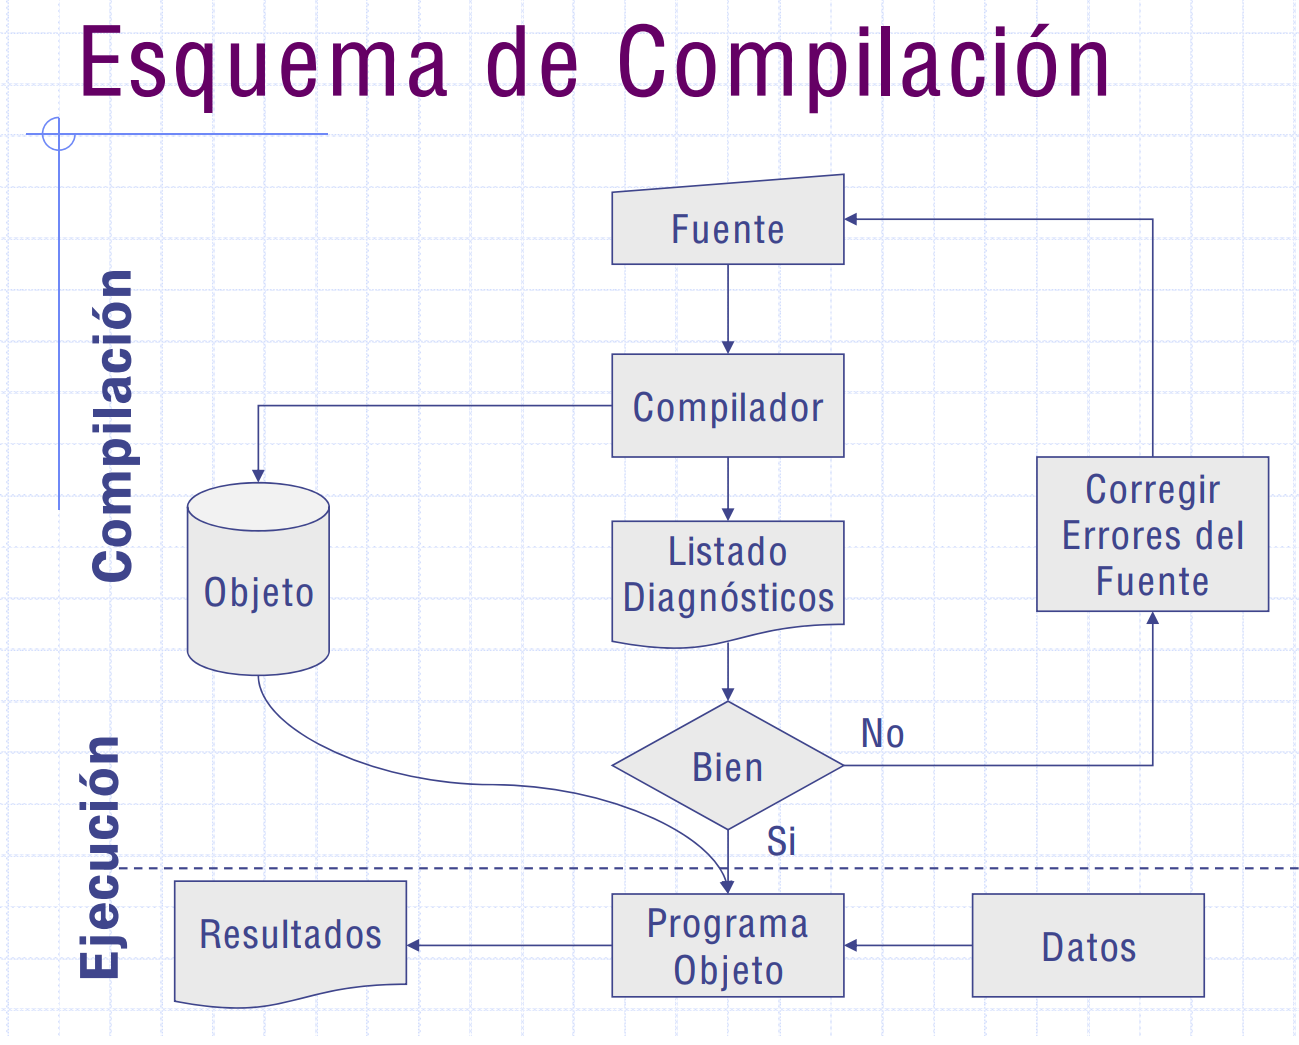
\includegraphics[scale=.15]{Untitled 9.png}
	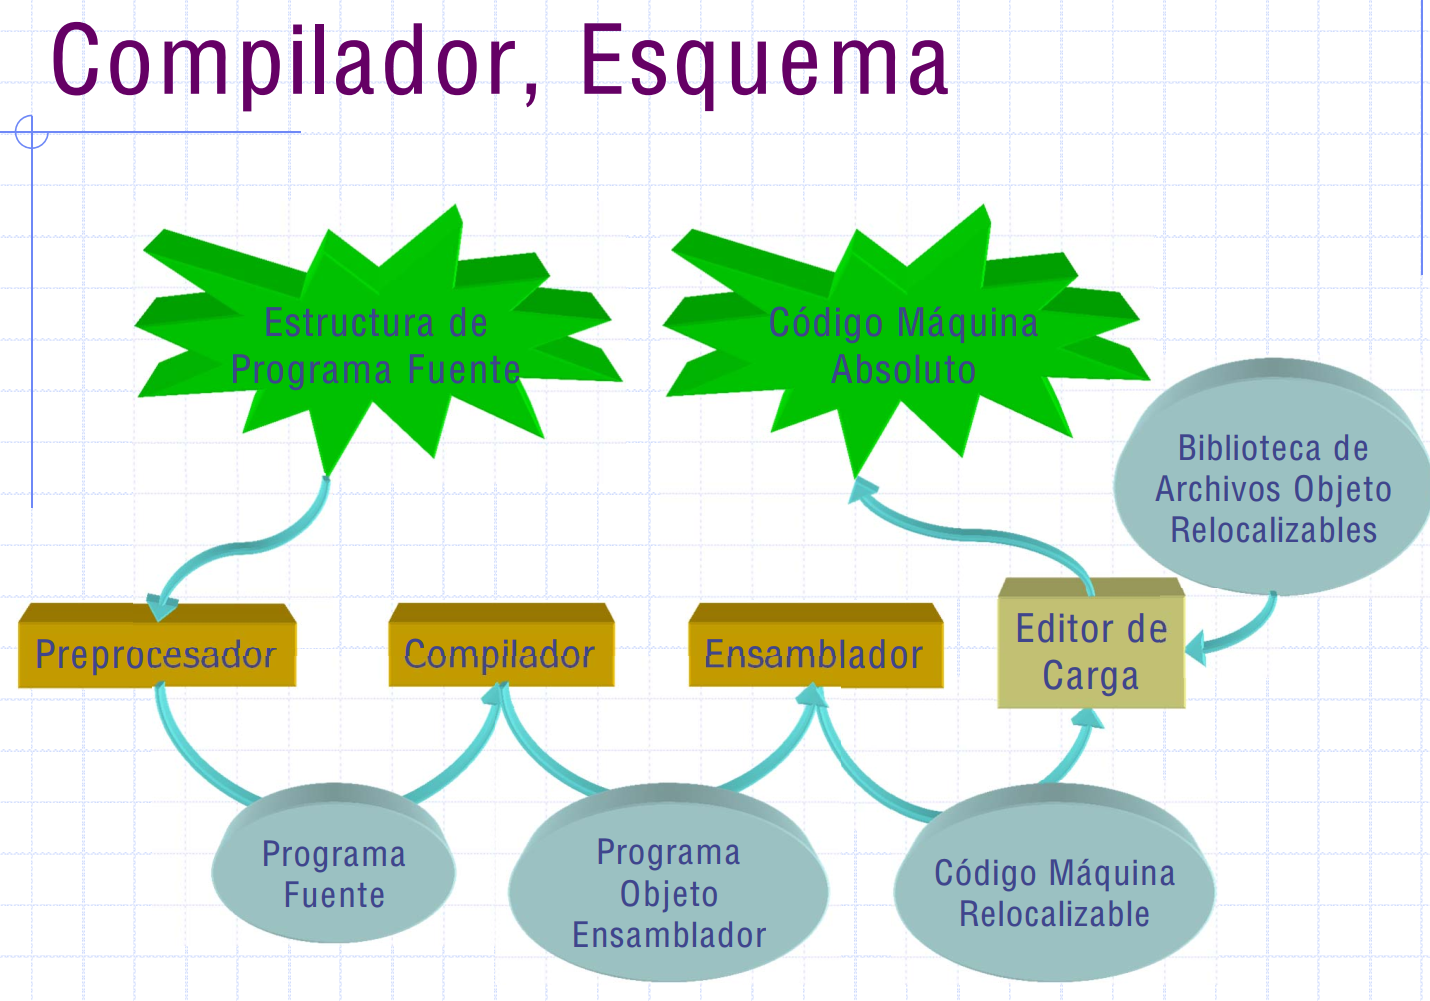
\includegraphics[scale=.15]{Untitled 10.png}}
\end{figure}



Antes del pasar al compilador se pasa al \textbf{preprocesador que hace
muchas funciones}, entre ellas, sustituir las variables constantes por
su valor y quita los comentarios. Cuando termina pasa el programa fuente
al compilador.

\begin{figure}[H]
	\ffigbox[\FBwidth]
	{\caption{Diagrama de Fases de un Compilador}}
	{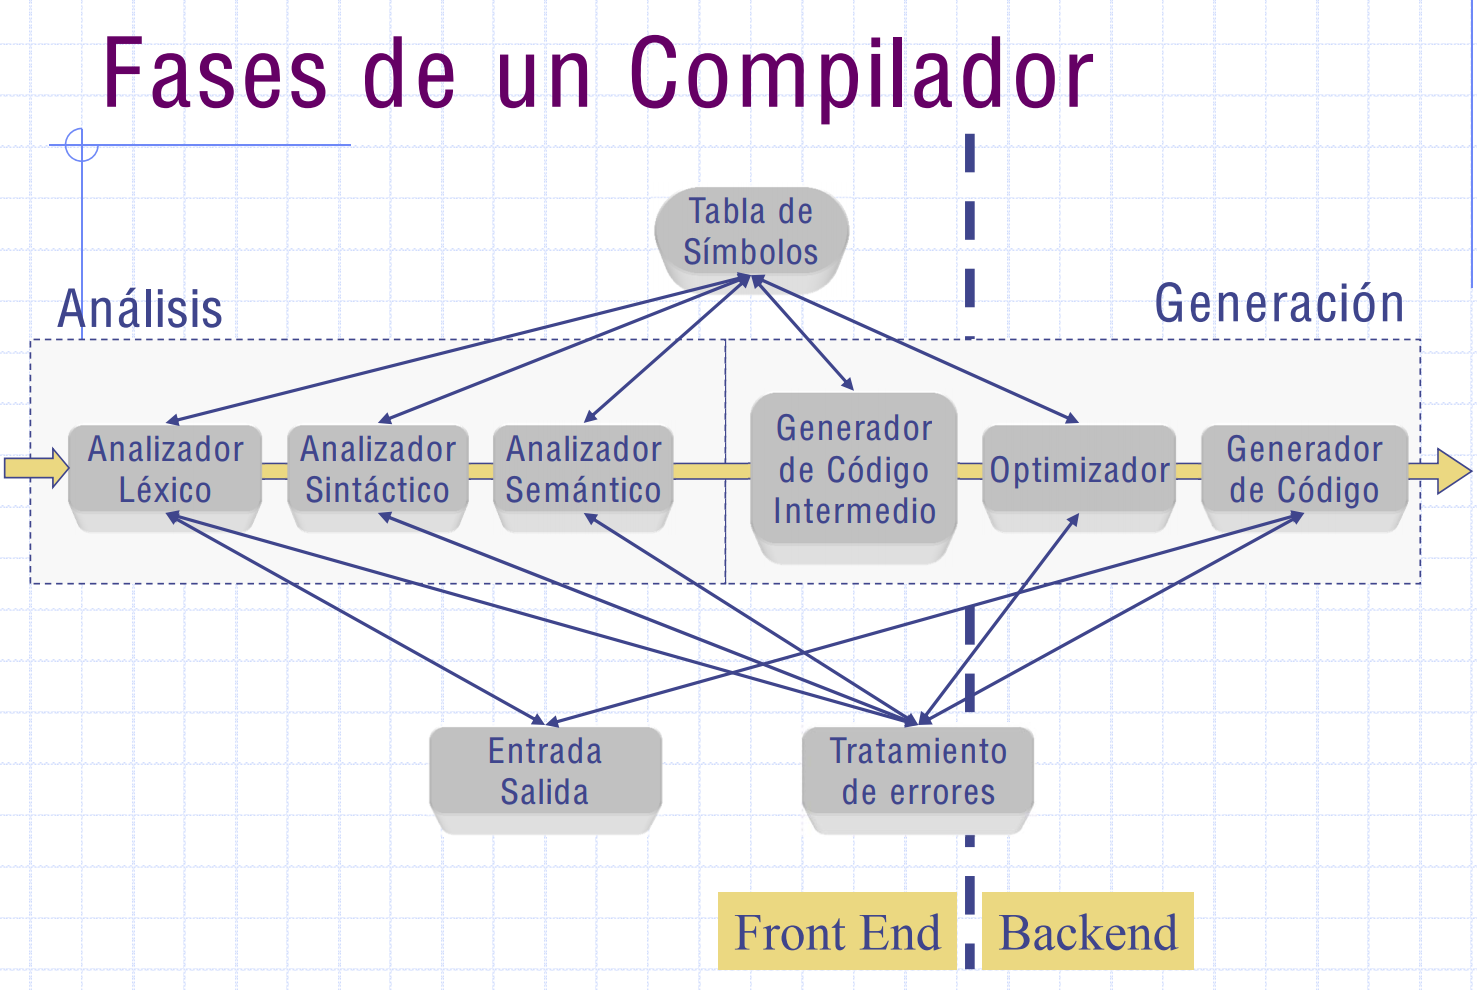
\includegraphics[scale=.27]{Untitled 11.png}}
\end{figure}

\textbf{Análisis}: Parte que solo depende de la estructura del lenguaje.
No depende de la arquitectura.

\textbf{Analizador léxico}: A este llegan directamente los datos, no al
resto. Su salida va al siguiente.

\textbf{Generación}: Depende de la arquitectura, pero no del lenguaje.

\textbf{Generador de código intermedio}: A veces se encuentra en
análisis y otras en generación.

\textbf{Analizador léxico (scanner)}: Convierte la entrada (y::= 3+b*3)
en Símbolos terminales (id op numo p id op num) de una gramática.

Análisis lineal: La cadena de entrada se lee de izquierda a derecha y se
agrupa en componentes léxicos (tokens)

\begin{figure}[H]
	\ffigbox[\FBwidth]
	{\caption{Diagrama Analizador Léxico}}
	{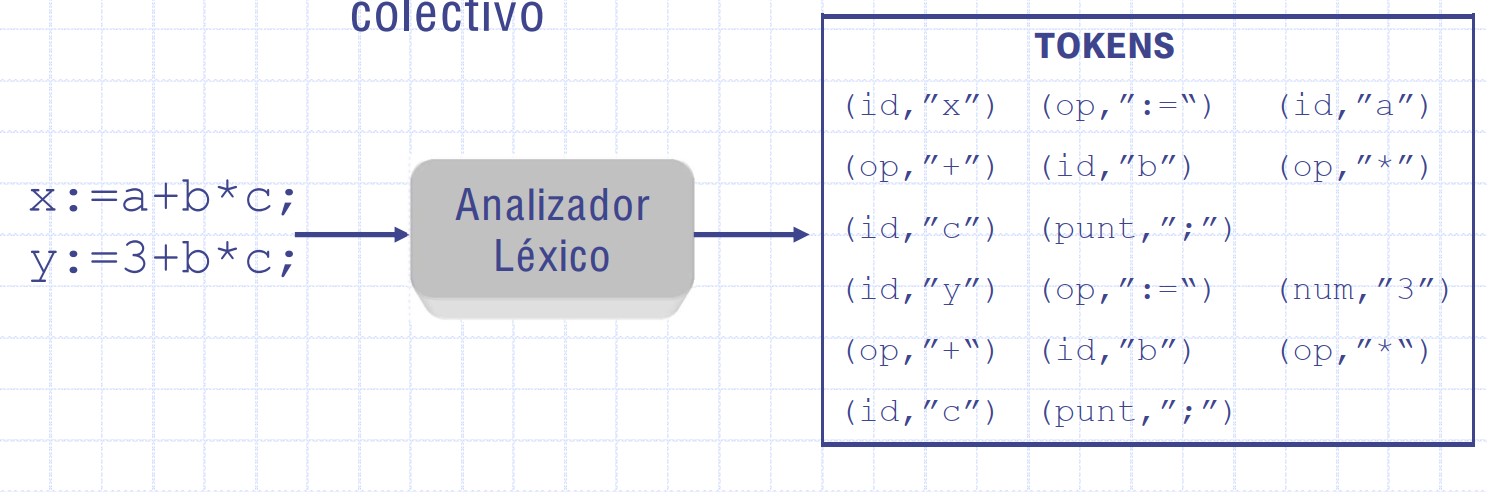
\includegraphics[scale=.25]{Untitled 12.png}}
\end{figure}

\textbf{Analizador sintáctico:} Agrupa los componentes léxico en frases
gramaticales que el compilador utiliza. A partir de los tokens produce
un árbol sintáctico.

\begin{itemize}
\item
  Recibe tokens → crea un árbol.
\item
  En las hojas tiene los terminales en la manera en la que identifica el
  token.
\end{itemize}

\begin{figure}[H]
	\ffigbox[\FBwidth]
	{\caption{Diagrama Analizador Sintáctico}}
	{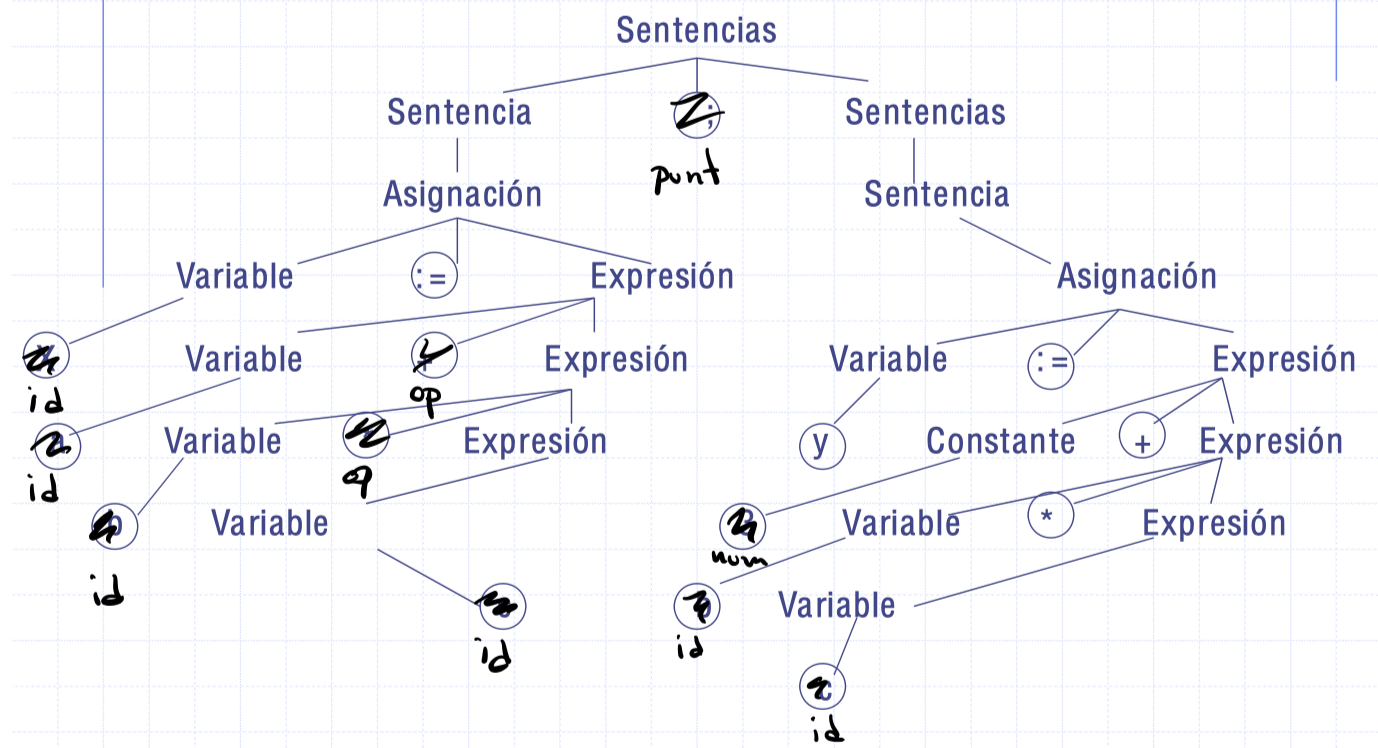
\includegraphics[scale=.25]{Untitled 13.png}}
\end{figure}

\textbf{Analizador semántico:} Busca errores semánticos, reúne
información de tipos; identifica operadores y operandos.

\begin{itemize}
\item
  Recibe el árbol sintáctico explícita o implícitamente, y trata de
  determinar si tiene sentido las distintas operaciones.

  Por ejemplo: Sumar un número y una cadena de caracteres.
\end{itemize}

\textbf{Generador de código}: A veces se encuentra en análisis y otras
en generación. Convierte el árbol en instrucciones, código
intermedio(ensamblador). El recorrido es importante ya que al generar
código no se ve la jerarquía. Por ejemplo: Primero se tienen que hacer
las operaciones antes de asignar el valor.

\begin{figure}[H]
	\ffigbox[\FBwidth]
	{\caption{Diagrama Generador de código}}
	{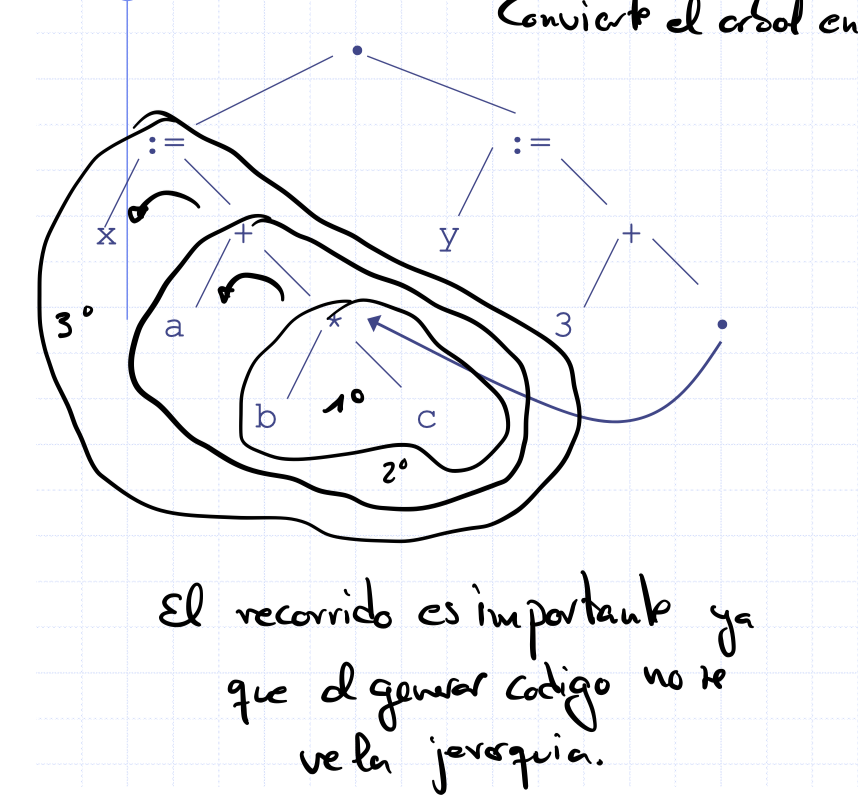
\includegraphics[scale=.25]{Untitled 14.png}}
\end{figure}

\textbf{Optimizador:} Trata de darse cuenta de subárboles comunes para
no repetir operaciones en las que no cambian variables. En vez de volver
a poner esa estructura apunta a ella.

\begin{figure}[H]
	\ffigbox[\FBwidth]
	{\caption{Diagrama Optimizador}}
	{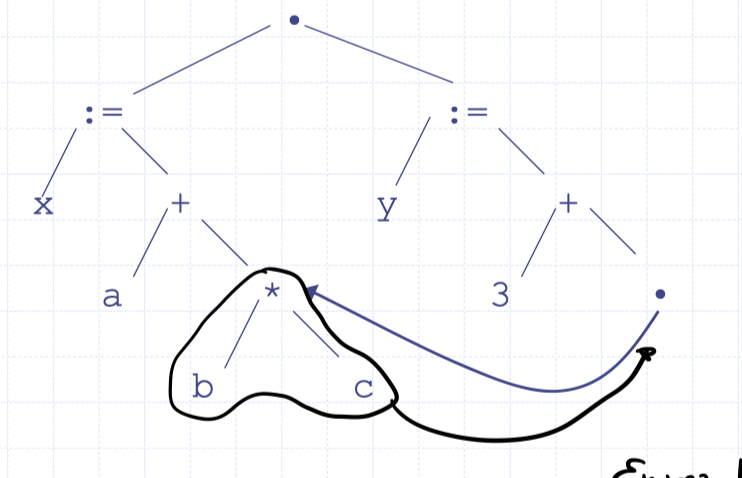
\includegraphics[scale=.3]{Untitled 15.png}}
\end{figure}

\textbf{Generador de código:} El uso de código intermedio reduce la
complejidad del desarrollo de compiladores. m front ends y n back-ends
comparten un código intermedio común.

\textbf{Front-end}: Etapa inicial. Fases que dependen del lenguaje
fuente y que son independientes de la máquina. Análisis léxico,
sintáctico, semántico y generación de código intermedio, manejo de
errores de cada parte.

\textbf{Back-end}: Etapa final. Fases que dependen de la máquina,
dependen del lenguaje intermedio. Optimización de código, generación de
código, operaciones con la tabla de símbolos.


\section{Diagramas de Tombstone}

Conjunto de piezas de puzzle útiles para razonar acerca de los
procesadores de lenguaje y los programas.

Está formado por piezas que deben encajar, encajan según unas reglas de
formación.

La máquina y el lenguaje deben coincidir.

\begin{figure}[H]
	\ffigbox[\FBwidth]
	{\caption{Diagrama Tombstone Programas y Máquinas}}
	{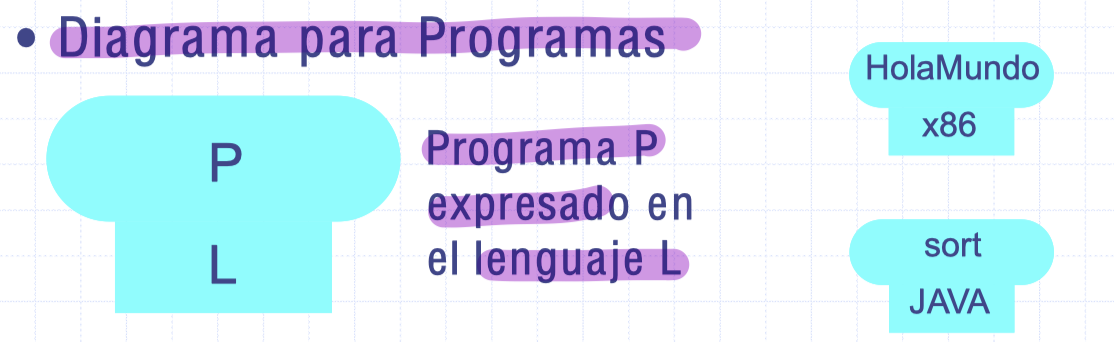
\includegraphics[scale=.17]{Untitled 16.png}
	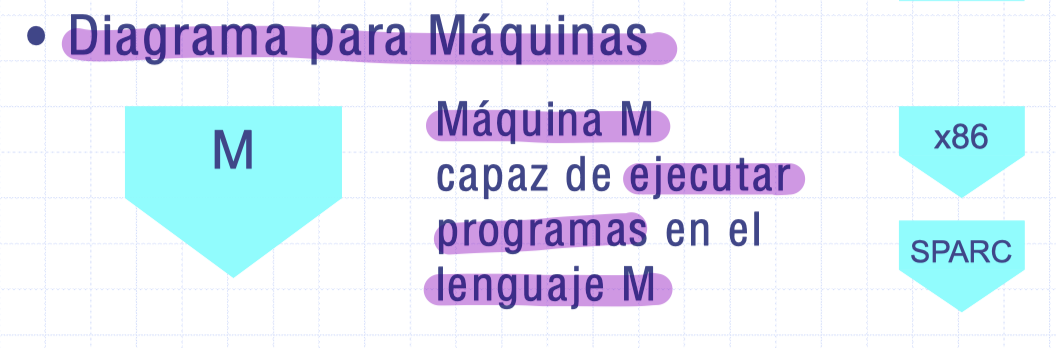
\includegraphics[scale=.17]{Untitled 17.png}}
\end{figure}

\begin{figure}[H]
	\ffigbox[\FBwidth]
	{\caption{Diagrama Tombstone Interpretes y Compiladores}}
	{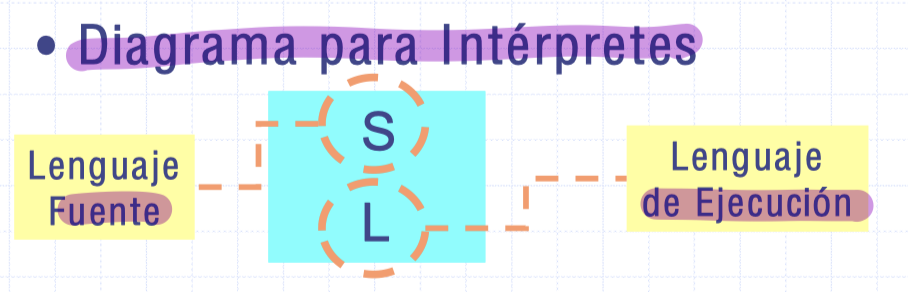
\includegraphics[scale=.2]{Untitled 18.png}
	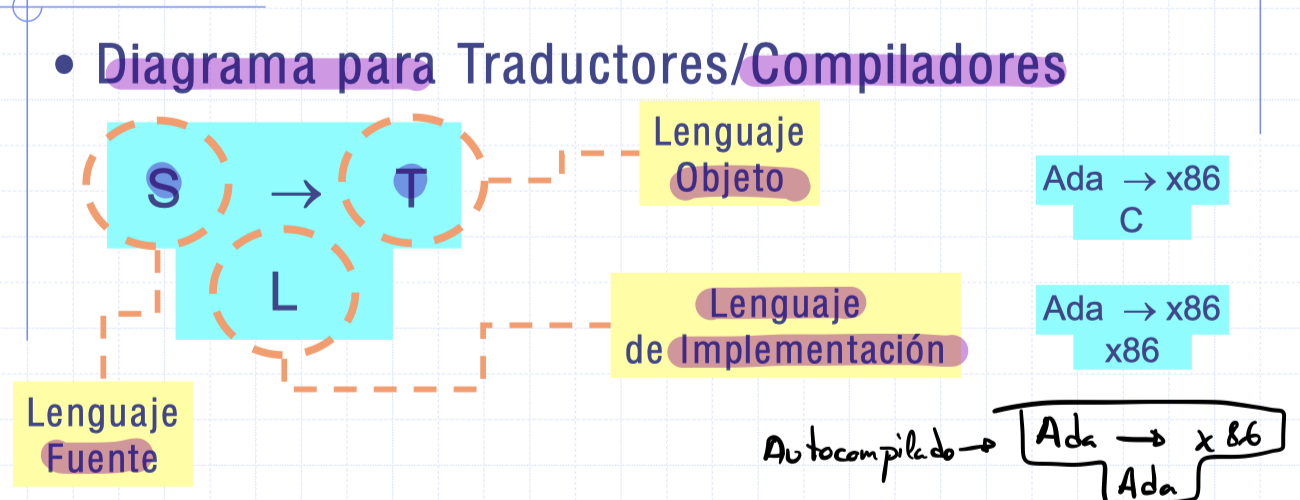
\includegraphics[scale=.13]{Untitled 19.png}}
\end{figure}

\begin{figure}[H]
	\ffigbox[\FBwidth]
	{\caption{Diagrama Maquinas Abstractas e Intérpretes}}
	{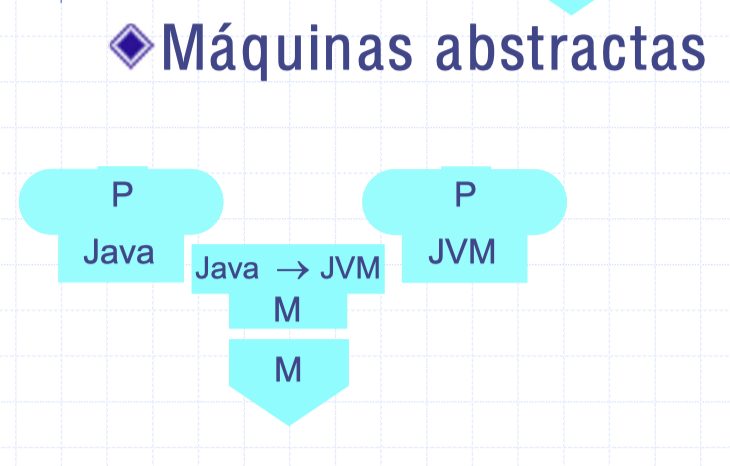
\includegraphics[scale=.2]{Untitled 20.png}
	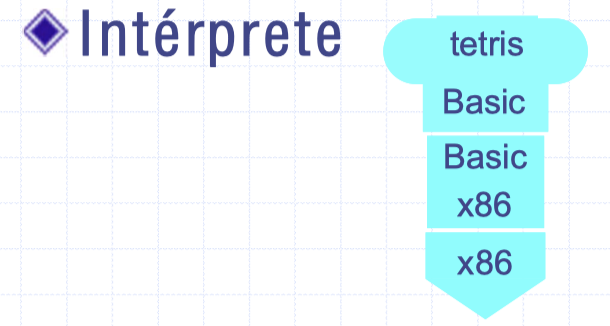
\includegraphics[scale=.2]{Untitled 21.png}}
\end{figure}

\begin{figure}[H]
	\ffigbox[\FBwidth]
	{\caption{Obtener un compilador rápido}}
	{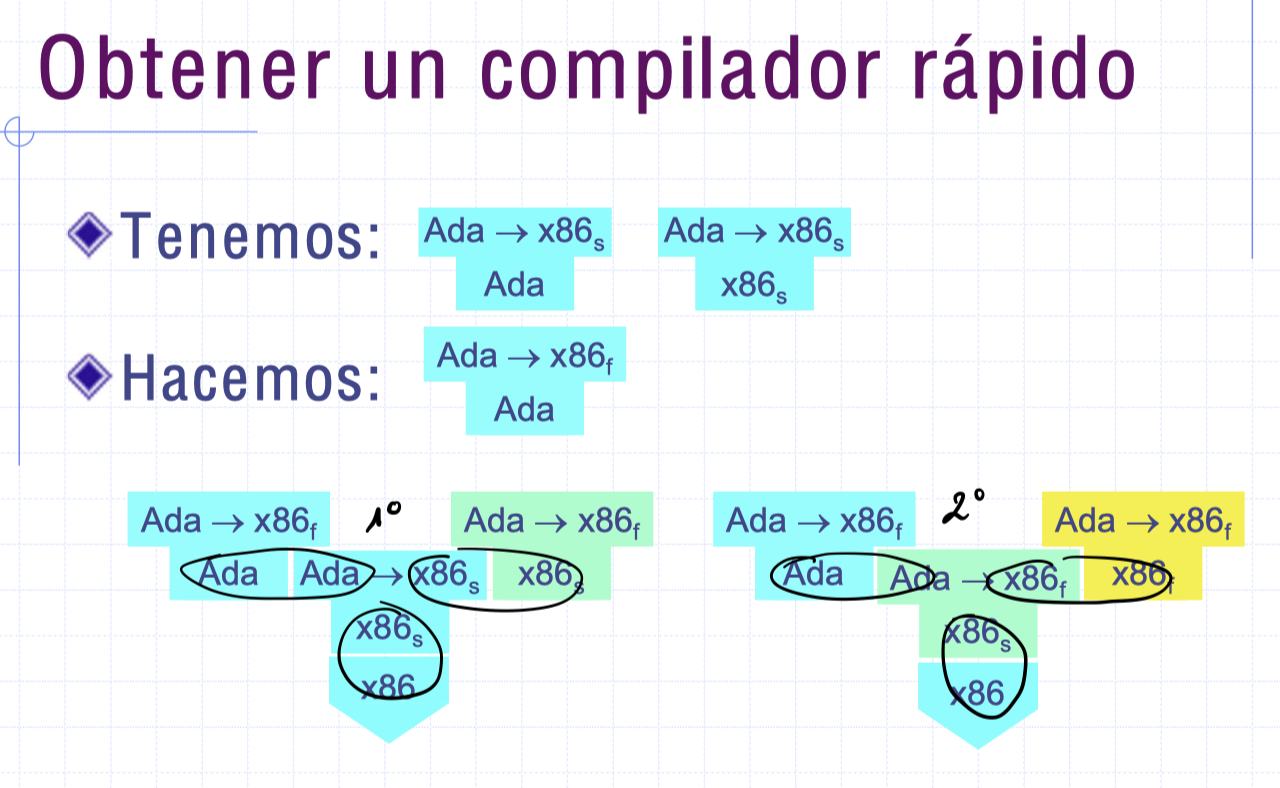
\includegraphics[scale=.15]{Untitled 22.png}
	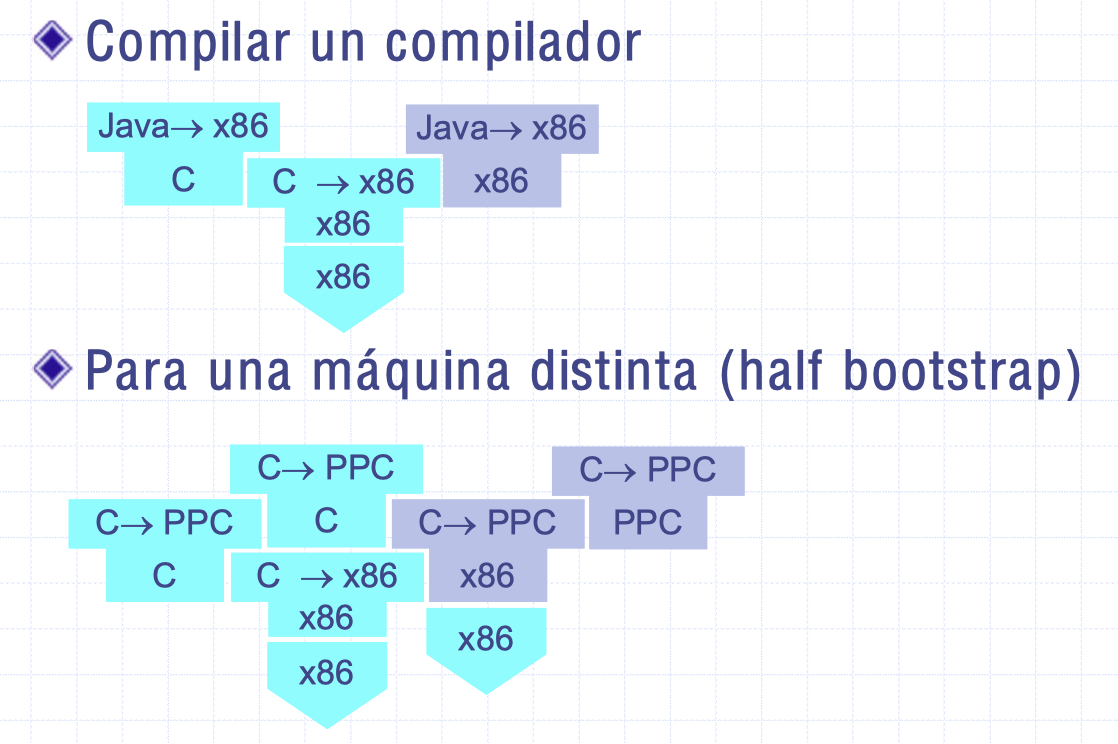
\includegraphics[scale=.15]{Untitled 23.png}}
\end{figure}

\begin{figure}[H]
	\ffigbox[\FBwidth]
	{\caption{Full Bootstrapping}}
	{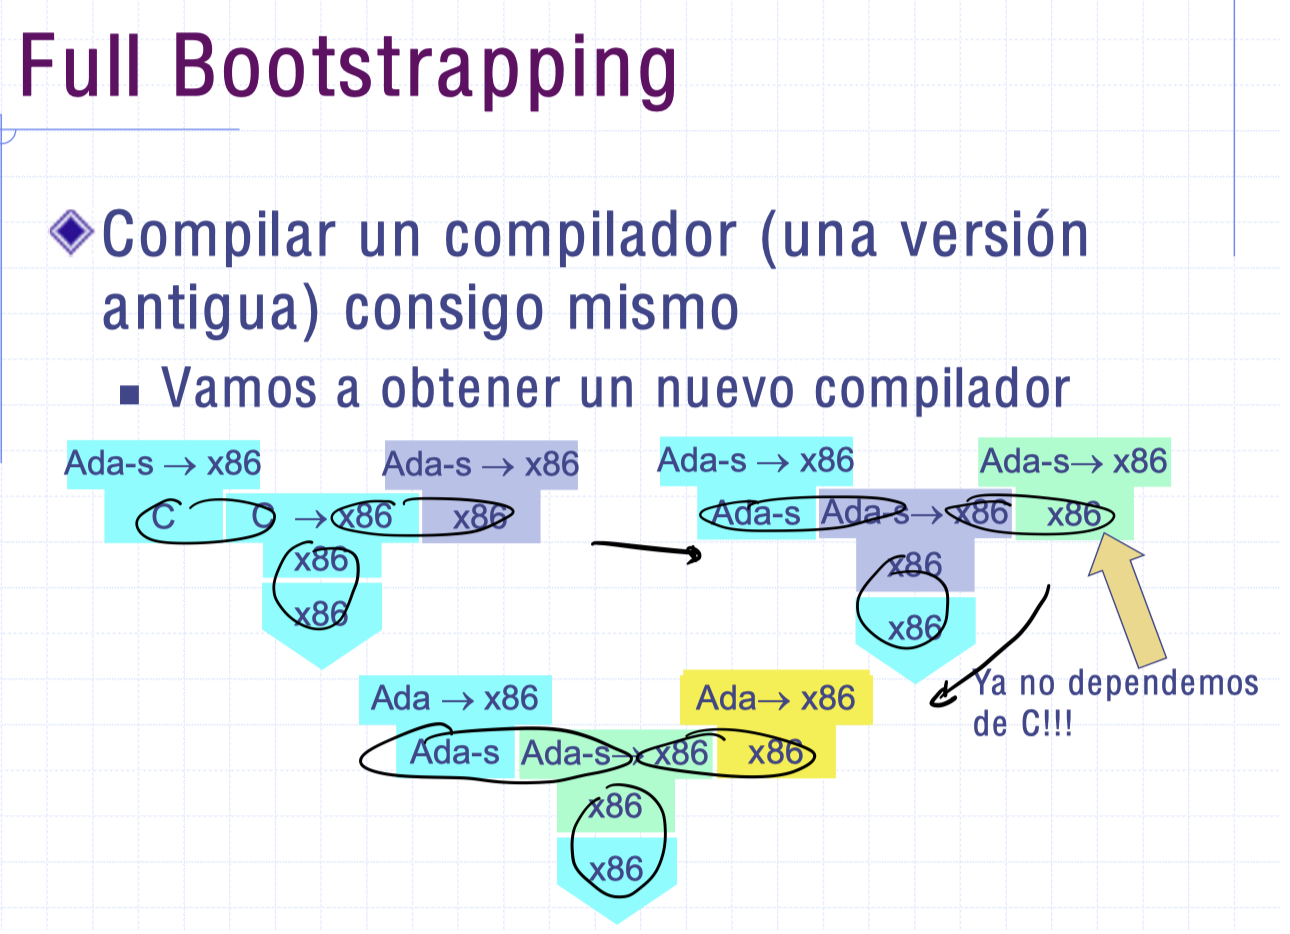
\includegraphics[scale=.2]{Untitled 24.png}}
\end{figure}

\begin{itemize}
	\item
	  Ejemplos:
\end{itemize}

\begin{figure}[H]
	\ffigbox[\FBwidth]
	{\caption{Ejemplo Full Bootstrapping}}
	{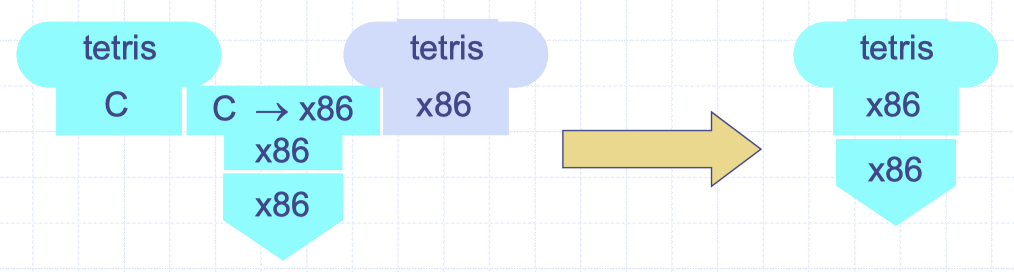
\includegraphics[scale=.2]{Untitled 25.png}}
	{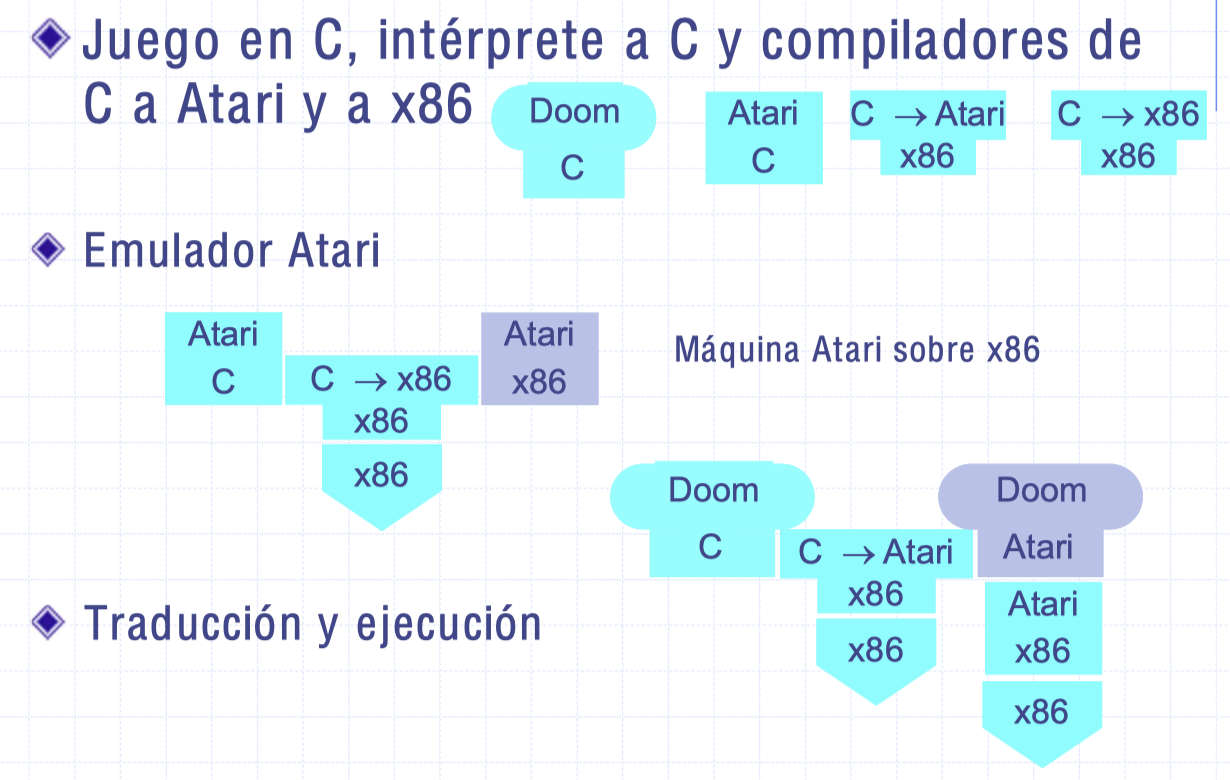
\includegraphics[scale=.2]{Untitled 26.png}}
\end{figure}

\chapter{Tema 2: Análisis Léxico}

\begin{figure}[H]
	\ffigbox[\FBwidth]
	{\caption{Diagrama AL}}
	{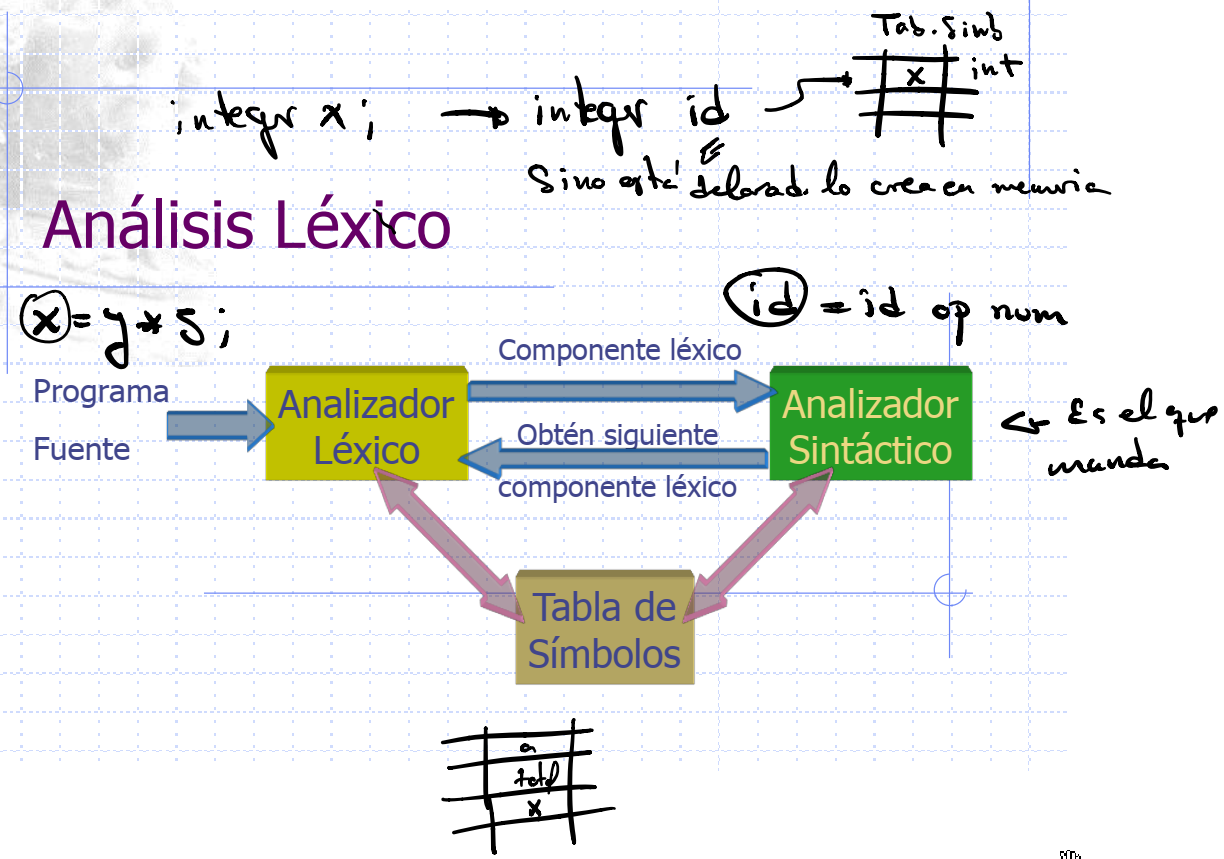
\includegraphics[scale=.25]{Untitled 27.png}}
\end{figure}

\section{Funciones del Análisis Léxico}

\textbf{Manejar el fichero fuente:} Leer los caracteres de la entrada.
Eliminar comentarios y delimitadores. Relacionar los mensajes de error
con las líneas del programa fuente.

\textbf{Interfaz con las otras fases de análisis:} Generar la secuencia
de componentes léxicos (tokens). Introducir los identificadores en la
\textbf{tabla de símbolos}. Manejar macros. pi→3,14

\textbf{Controlar si es de formato libre o no:} Libre: PASCAL. No libre:
FORTRAN.


\section{Aspectos del Análisis Léxico}

\textbf{Diseño más sencillo:} Los símbolos que trata el scanner se
describe con una gramática más simple que la del parser.

\textbf{Mejora la eficiencia:} Gran parte del tiempo de compilación se
consume en la lectura y exploración.

\textbf{Mejora la portabilidad:} Se pueden tener varias versiones del
scanner una para distintos códigos.

\textbf{Tokens}: Unidades sintácticas de un lenguaje. Símbolos
terminales de una gramática, identificadores, palabras reservadas.

\begin{itemize}

\item
  num es el token.
\end{itemize}

\textbf{Categoría:}

\begin{itemize}
\item
  \textbf{Palabras reservadas}: IF, THEN, DO\ldots{}
\item
  \textbf{Identificadores}: main, suma, identificadores\ldots{}
\item
  \textbf{Símbolos especiales}: Como \textless, \textgreater\ldots{}
\item
  \textbf{Constantes y literales.}
\end{itemize}

\textbf{Lexema:} Secuencias válidas para un token. Secuencia de
caracteres del código fuente que son identificados como un token
específico.

\begin{itemize}

\item
  El lexema de num son los valores que puede tomar: 12, 34, 480
\end{itemize}

\textbf{Atributos:} Información adicional que tiene el token.

\begin{itemize}

\item
  id.lexema=``x'' id.tipo id.ámbito
\end{itemize}

\textbf{Patrón:} Define la secuencia de caracteres válidos para un
tokens, formato de los lexemas.

\begin{itemize}
\item
  \([0-9]^+\) Naturales \(-?[0-9]^+\) Enteros de -9 a 9
\item
  El + al final, indica que hay 1 o más ocurrencias. Para poner
  determinados símbolos se ponen ""
\end{itemize}

\textbf{Especificar tokens:} Con expresiones regulares, patrones, o
Autómatas Finitos.

\begin{itemize}
\item
  Los elementos básicos en un lenguaje deben ser tokens.
\item
  Se pueden usar Expresiones regulares o Autómatas Finitos.
\end{itemize}

\textbf{Tabla de símbolos:} Almacenan la correspondencia entre tokens y
lexemas, en muchos lenguajes hay palabras claves (reservadas) que no se
pueden declarar una variable para ello se almacena en la tabla.

\begin{itemize}

\item
  Los atributos de los identificadores se pueden guardar en la tabla de
  símbolos. Los otros en otra tabla.
\end{itemize}

\begin{figure}[H]
	\ffigbox[\FBwidth]
	{\caption{Diagramas A. Lexico}}
	{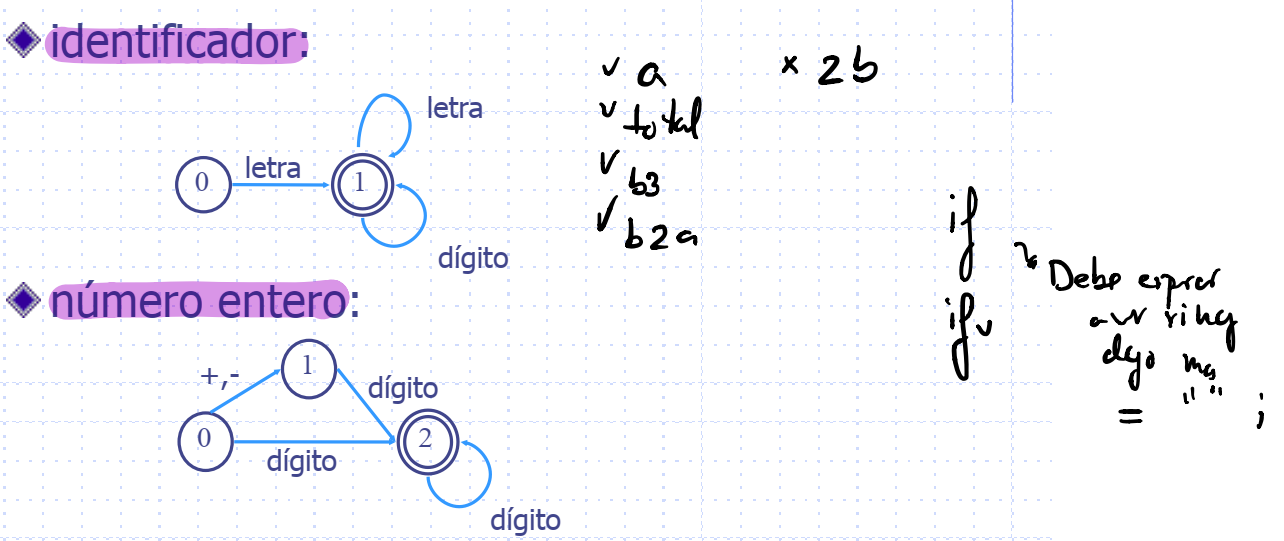
\includegraphics[scale=.2]{Untitled 28.png}
	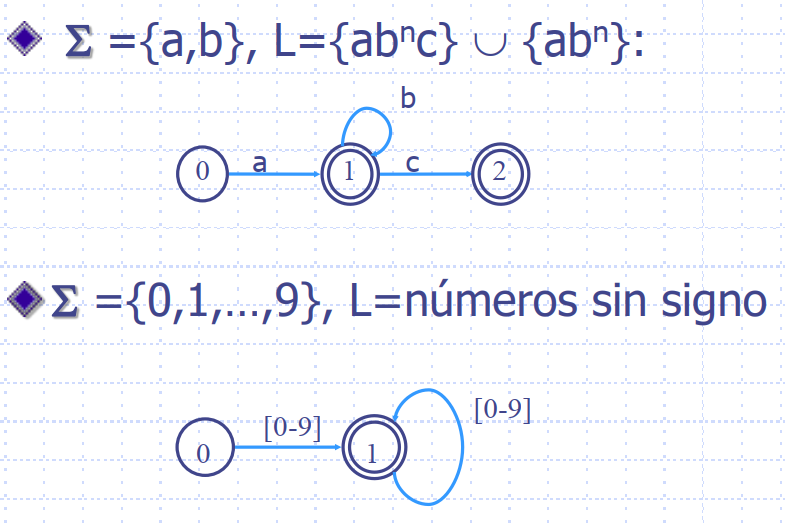
\includegraphics[scale=.2]{Untitled 29.png}}
\end{figure}

Un AF no devuelve el token, se usa otra cosa para que nos dé el token
cuando reconoce símbolos.

Nosotros vamos a usar DT para representar.


\section{Diagrama de Transiciones - DT}

\textbf{Definir formalmente un AL es hacer los DT de los tokens} (ojo
con los separadores que llevan a finales, si no hay nada, que no salga)

Se usa para especificar el funcionamiento de un Analizador Léxico
mediante un AFD. \textbf{UNO POR TOKEN}

Se diferencian porque el DT reconoce un token cuando reconoce un
delimitador y devuelve entonces el token. \textbf{Lee caracteres hasta
completar un token entonces: Devuelve el token leído} y Deja el buffer
listo para la siguiente llamada.

No tiene estados de error. De los estados de aceptación no salen
transiciones, necesita una transición más que no pertenece al token, que
le hace salir y devolver el token.

Esto quiere decir que aquellos estados que son terminales y pueden
transitar a otro estado tengan una transición para otro tipo de carácter
que hace que salga como final.

\begin{figure}[H]
	\ffigbox[\FBwidth]
	{\caption{Ejemplo de Diagrama de Transiciones}}
	{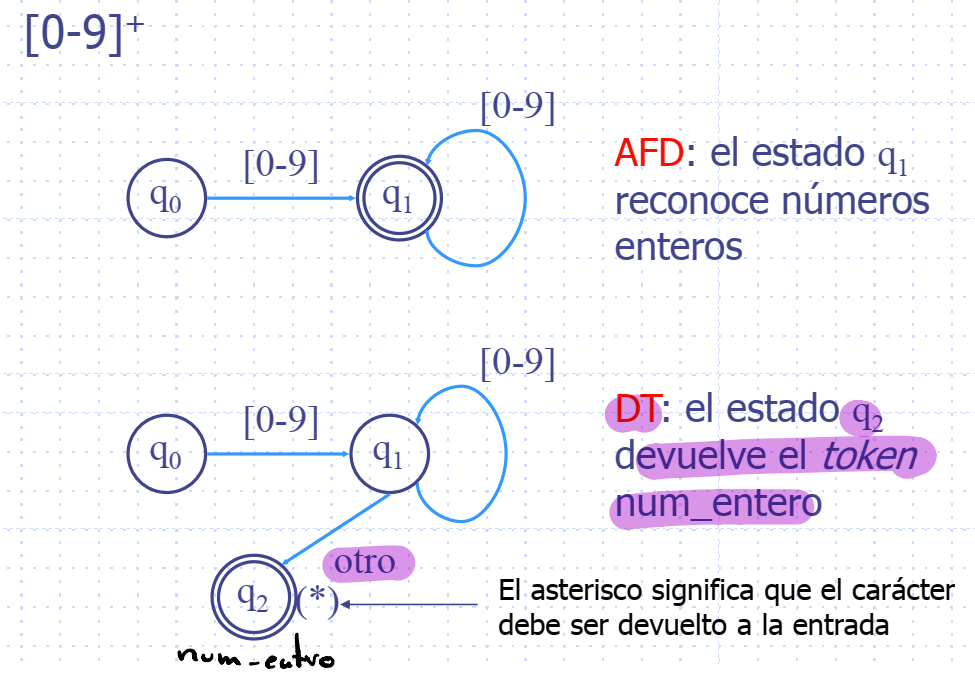
\includegraphics[scale=.25]{Untitled 30.png}}
\end{figure}

\section{Construcción de un AFD para AL}

Normalmente se parte de representación de las reglas de tokens con
expresiones regulares.

\begin{enumerate}
\def\labelenumi{\arabic{enumi}.}

\item
  Toda expresión regular tiene un AFND asociado.
\item
  Construir un AFD para el mismo lenguaje del AFND
\item
  Optimización del AFD.
\end{enumerate}


\section{Tabla de Transiciones de DT}

\begin{figure}[H]
	\ffigbox[\FBwidth]
	{\caption{Diagrama Tabla de Transiciones}}
	{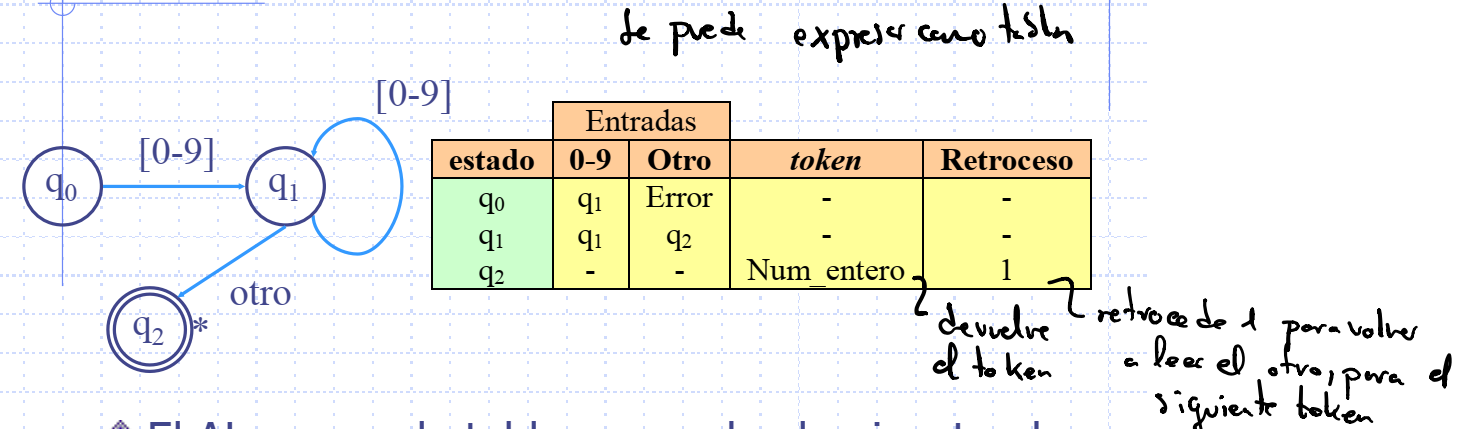
\includegraphics[scale=.25]{Untitled 31.png}}
\end{figure}

\section{Autómata programado}

Es la manera de programar un Analizador Léxico.

Representa directamente con un programa al DT en cuestión.

\begin{figure}[H]
	\ffigbox[\FBwidth]
	{\caption{Diagrama Optimizador}}
	{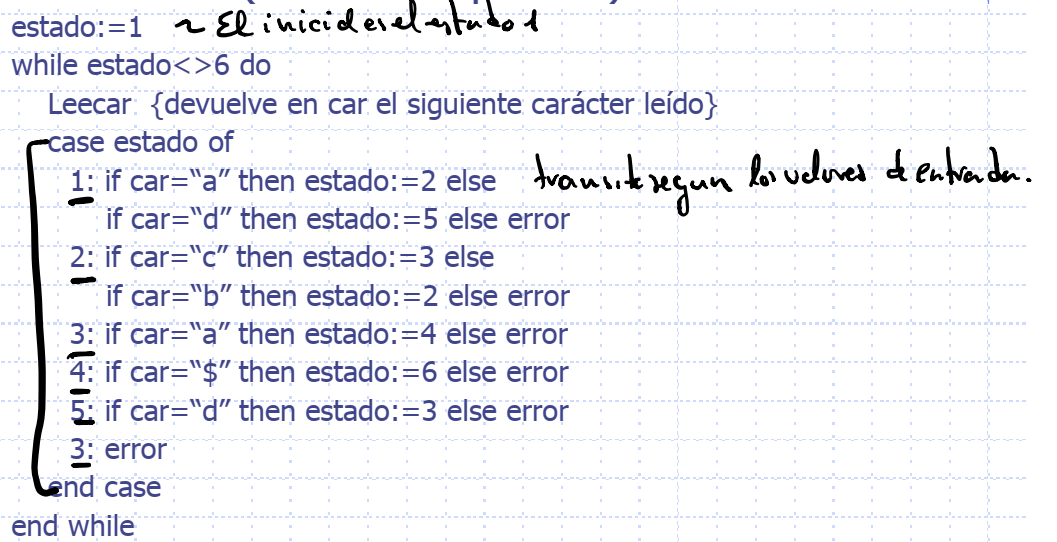
\includegraphics[scale=.3]{Untitled 32.png}}
\end{figure}

\section{Implementación de un AL}

\subsection{Utilizando un generador de Analizadores Léxicos (es lo que usaremos)}

\begin{itemize}
\item
  \textbf{Ventajas}: Comodidad y Rapidez de desarrollo.
\item
  \textbf{Inconvenientes}: Ineficiencia.
\item
  \textbf{Recomendación}: Ordenar las reglas de acuerdo con la frecuencia
  de utilización.
\end{itemize}


\subsection{Utilizando ensamblador}

\begin{itemize}

\item
  \textbf{Ventajas}: Mas eficiente y compacto.
\item
  \textbf{Inconvenientes}: Mas difícil de desarrollar y Dificultad de
  mantenimiento de código generado.
\end{itemize}


\subsection{Utilizando un lenguaje de alto nivel}

\begin{itemize}
\item
  \textbf{Ventajas}: Eficiente y Compacto.
\item
  \textbf{Inconveniente}: Realizar todo a mano.
\item
  Técnicas:

  \begin{itemize}
  \item
    \textbf{Programación}: Muy eficiente.

    \begin{itemize}
    
    \item
      \textbf{Controlado por tablas}: Código pequeño, general y
      manejable.
    \end{itemize}
  \end{itemize}
\end{itemize}


\section{Programación de un AL}

\textbf{Dos punteros} de lectura:

\begin{itemize}
\item
  \textbf{Puntero actual}: El ultimo carácter aceptado.
\item
  \textbf{Puntero de búsqueda}: El ultimo carácter leído.
\end{itemize}

\begin{figure}[H]
	\ffigbox[\FBwidth]
	{\caption{Diagrama punteros AL}}
	{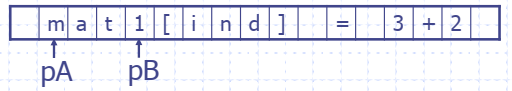
\includegraphics[scale=.3]{Untitled 33.png}}
\end{figure}

\textbf{Funciones de lectura}: GetChar(avanza uno del avanzado y da el
valor), Fail(Mueve el puntero avanzado de vuelta al aceptado),
Retract(mueve el puntero avanzado uno atrás) y Accept(mueve el puntero
actual hasta el avanzado).

\textbf{Primitivas}: IsLetter(letra), IsDigit(número) y
IsDelimiter(separadores).

\textbf{Acciones}: InstallName(introduce un nombre en la tabla de
símbolos).


\section{Errores Léxicos}

Hay pocos detectables por el analizador léxico.

\textbf{Detectables, según el diseñador:}

\begin{itemize}

\item
  Número de caracteres de los identificadores.
\item
  Caracteres ilegales.
\item
  Otros, como admitir números sin la parte entera.
\item
  Cadena que no concuerda con ningún token.
\end{itemize}

\textbf{En caso de error:}

\begin{enumerate}
\def\labelenumi{\arabic{enumi}.}

\item
  Anotar el error, indicarlos.
\item
  Recuperarme del error para continuar con el análisis. Ignorar, Borrar,
  Insertar o Corregir.
\item
  Seguir.
\end{enumerate}


\section{Identificación de palabras reservadas}

Mediante \textbf{resolución implícita}, todas identificadas en el
comienzo de la tabla de símbolos, o \textbf{resolución explícita},
usando patrones para las palabras reservadas.


\section{Prioridad de los tokens}

\textbf{Criterio}: Se utilizan heurística para dar prioridad al token
que concuerda con \textbf{el lexema más largo}.

\textbf{En el caso se puede concordar a varios tokens} se asocia al que
esté \textbf{en primer lugar}.

\begin{figure}[H]
	\ffigbox[\FBwidth]
	{\caption{Diagrama Prioridad de los tokens}}
	{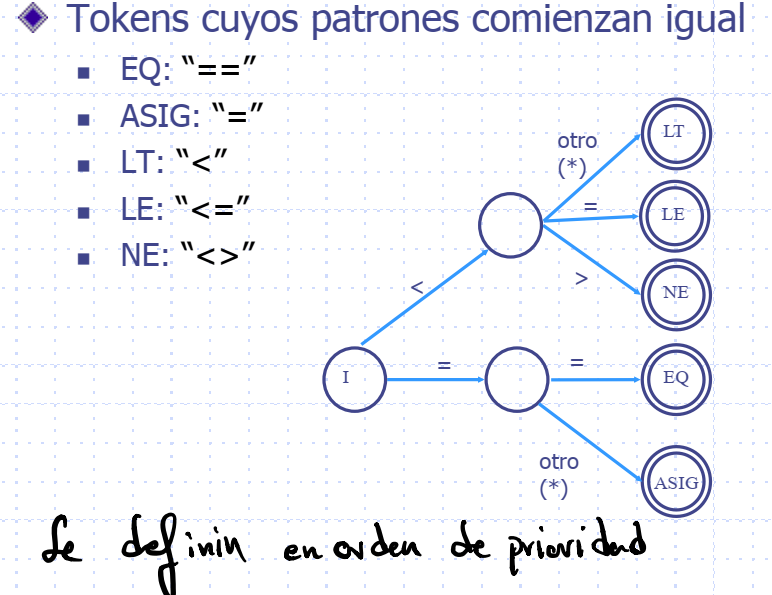
\includegraphics[scale=.3]{image-20210305191616426.png}
	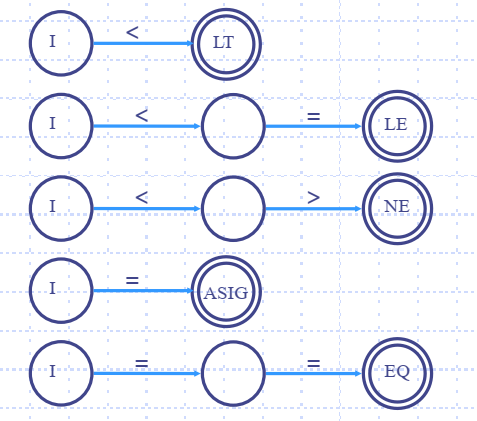
\includegraphics[scale=.3]{image-20210305191651759.png}}
\end{figure}

\section{AL y Lenguajes de Programación}

El \textbf{AL agrupa caracteres para formar tokens}, por tanto, es
importante definir el ``delimitador''.

\begin{itemize}

\item
  Carácter que \textbf{delimita el token sin pertenecer} a él.
\end{itemize}

Otro concepto importante es el de ``\textbf{palabra reservada}''

\begin{itemize}

\item
  El lenguaje \textbf{prohíbe el uso libre al programador de
  determinadas palabras} que tienen un significado específico y único en
  el lenguaje
\end{itemize}

\textbf{Lenguajes según uso de delimitadores y palabras reservadas:}

\begin{itemize}

\item
  \textbf{Delimitadores blancos; con palabras reservadas}

  \begin{itemize}
  
  \item
    Caso más sencillo de lenguaje (PASCAL, COBOL)
  \end{itemize}
\item
  \textbf{Delimitadores blancos; sin palabras reservadas}

  \begin{itemize}
  
  \item
    PL/I
  \end{itemize}
\item
  \textbf{Blancos se ignoran; sin palabras reservadas}

  \begin{itemize}
  
  \item
    El tipo más difícil de lenguaje, aparecen ambigüedades (FORTRAN)
  \item
    El espacio en blanco se elimina con un preprocesado.
  \item
    El AL tiene que retroceder y comenzar de nuevo.
  \end{itemize}
\end{itemize}

\section{Ejemplo de crear un AL y ASI}

\begin{figure}[H]
	\ffigbox[\FBwidth]
	{\caption{Ejemplo de crear un AL y ASI I}}
	{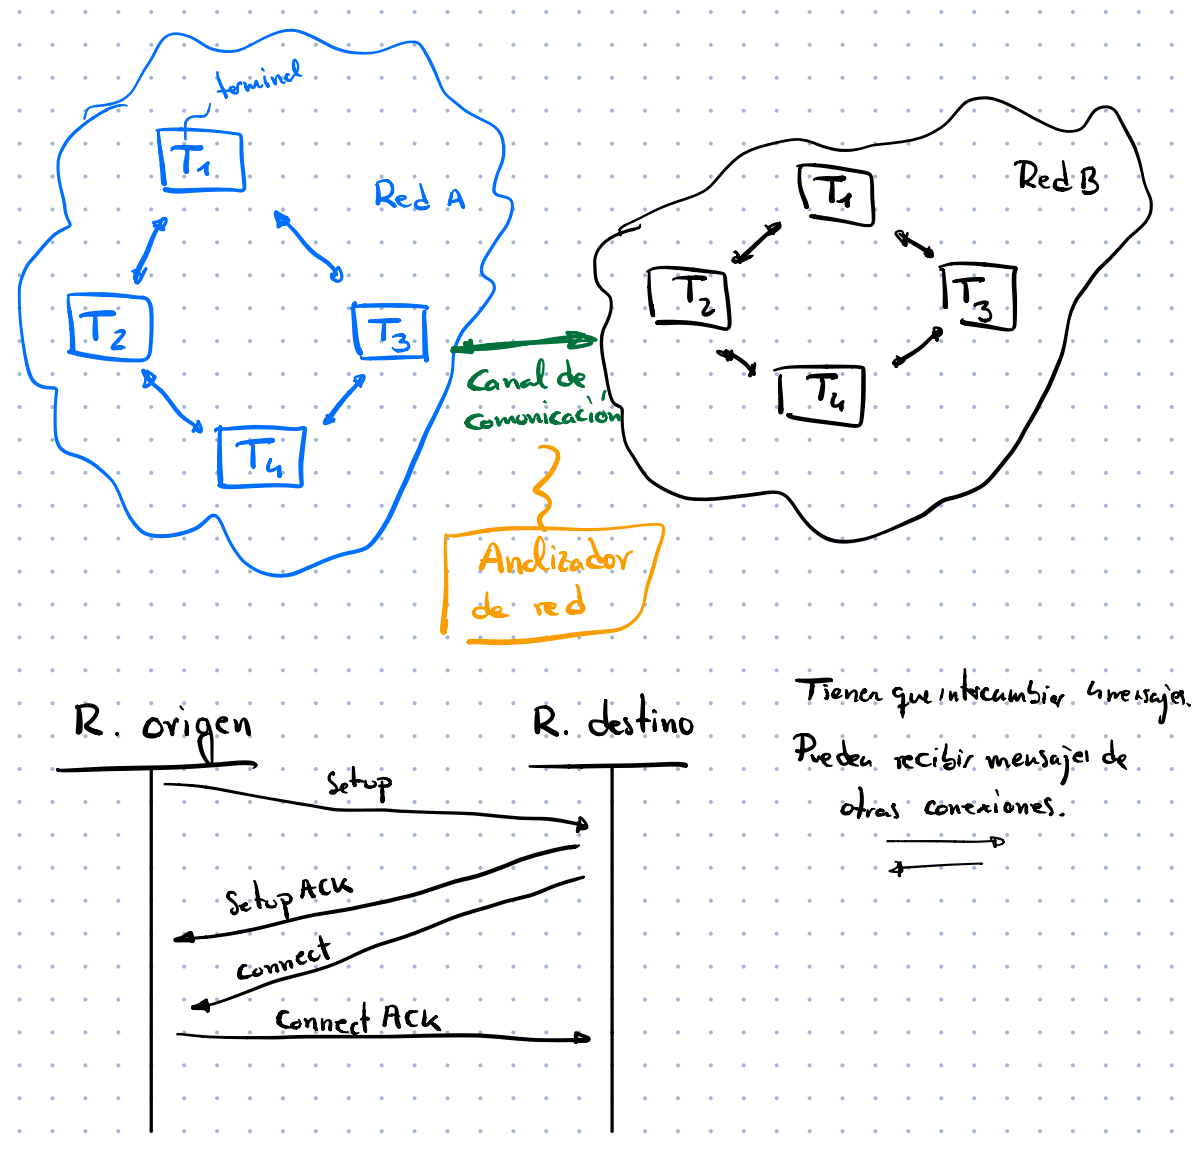
\includegraphics[scale=.2]{image-20210305192603381.png}}
\end{figure}

\begin{figure}[H]
	\ffigbox[\FBwidth]
	{\caption{Ejemplo de crear un AL y ASI II}}
	{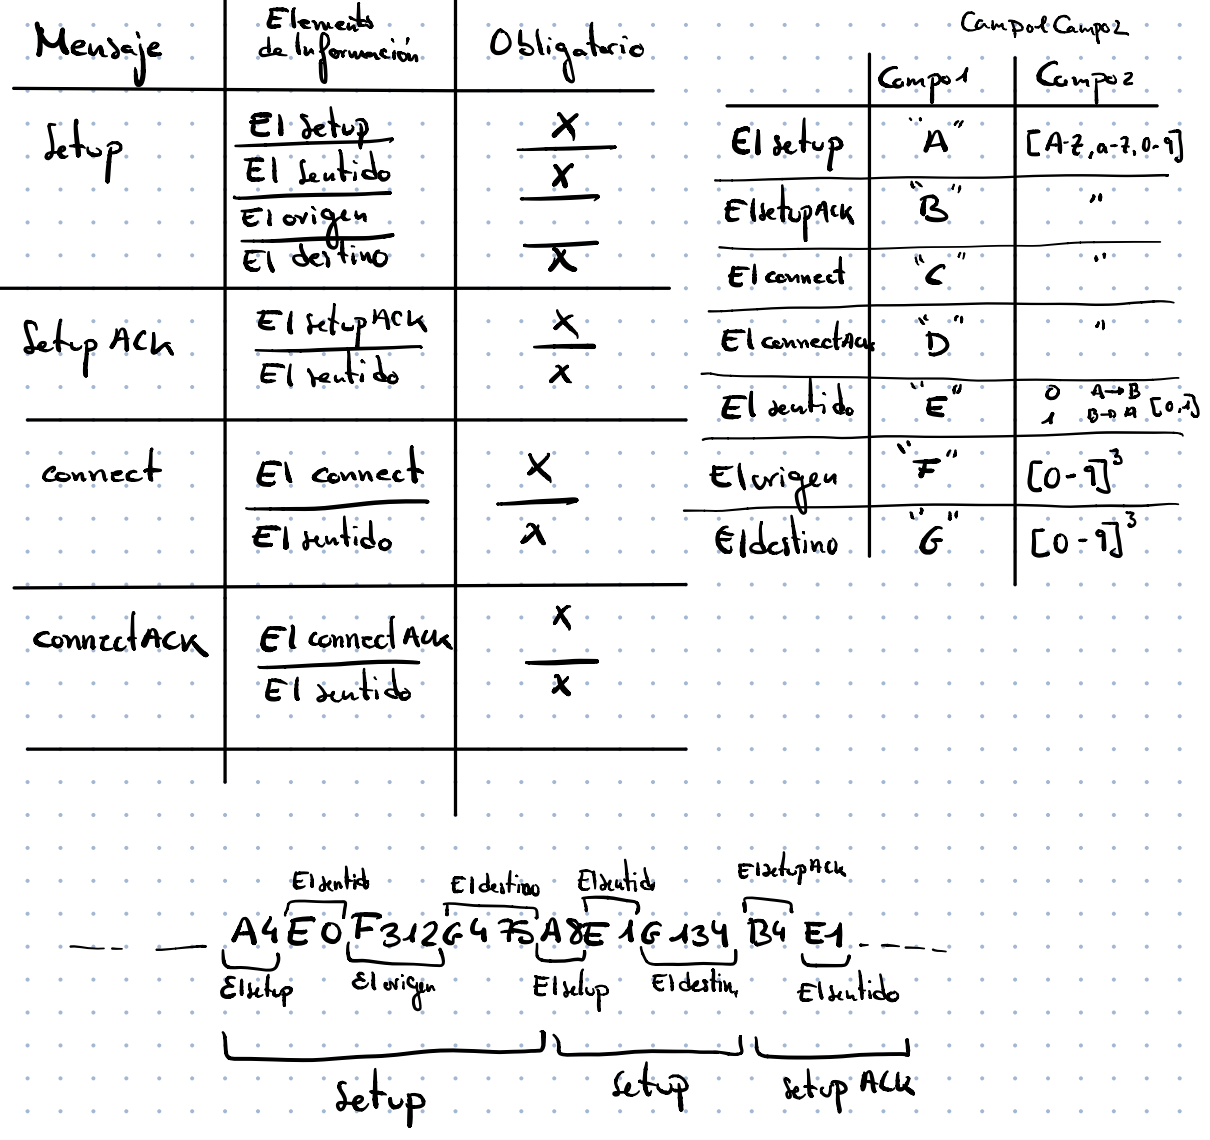
\includegraphics[scale=.3]{image-20210305192620642.png}}
\end{figure}

\begin{figure}[H]
	\ffigbox[\FBwidth]
	{\caption{Ejemplo de crear un AL y ASI III}}
	{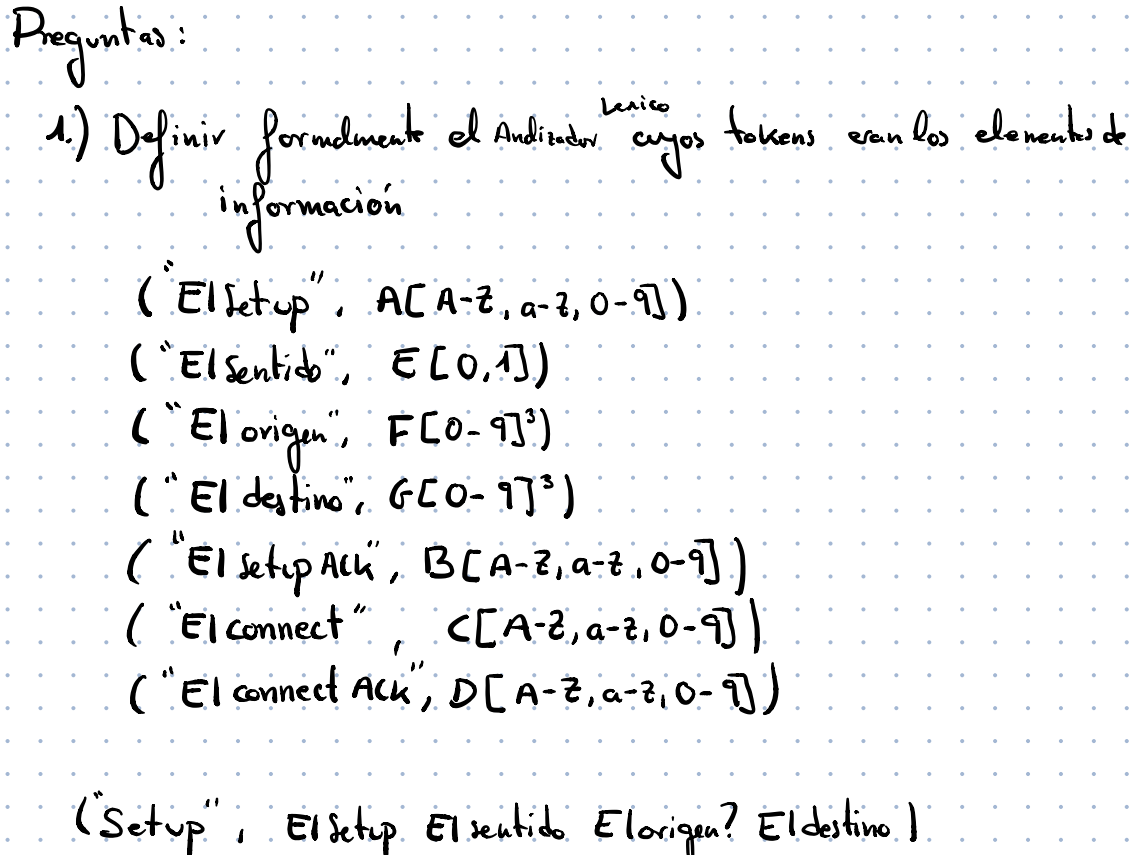
\includegraphics[scale=.2]{image-20210305192648153.png}}
\end{figure}

\begin{figure}[H]
	\ffigbox[\FBwidth]
	{\caption{Ejemplo de crear un AL y ASI IV}}
	{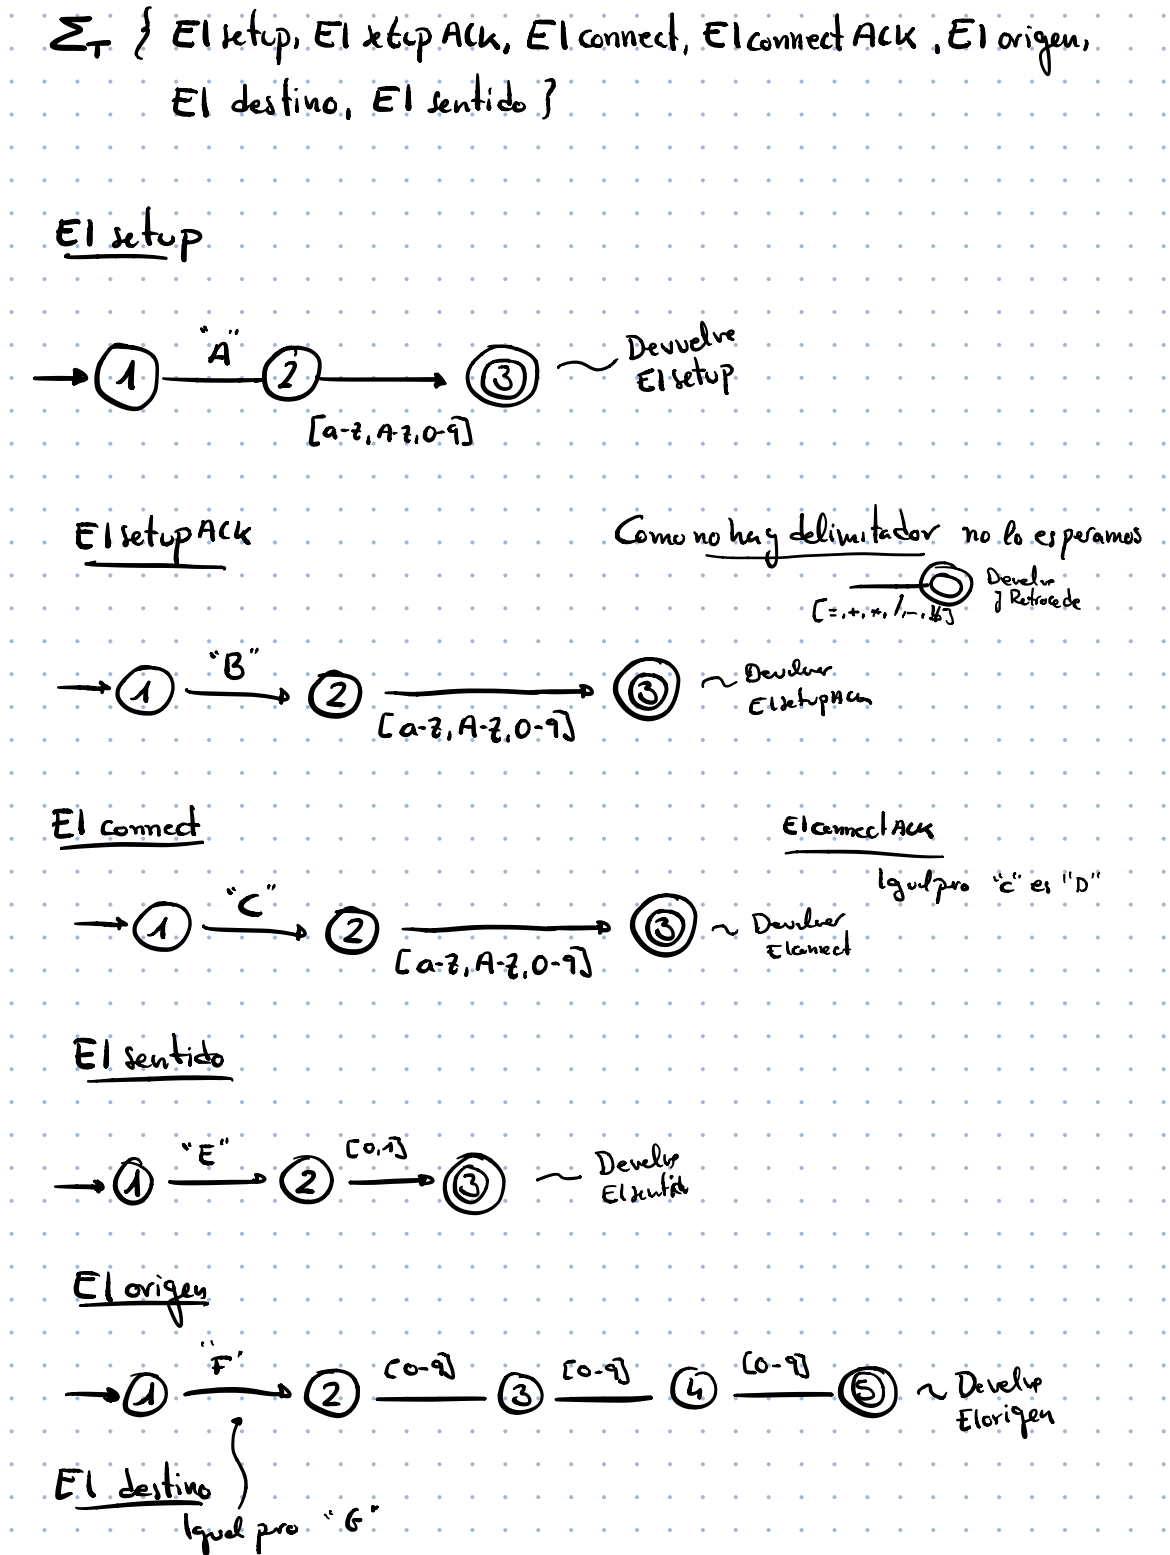
\includegraphics[scale=.25]{image-20210305192718592.png}}
\end{figure}

\begin{figure}[H]
	\ffigbox[\FBwidth]
	{\caption{Ejemplo de crear un AL y ASI V}}
	{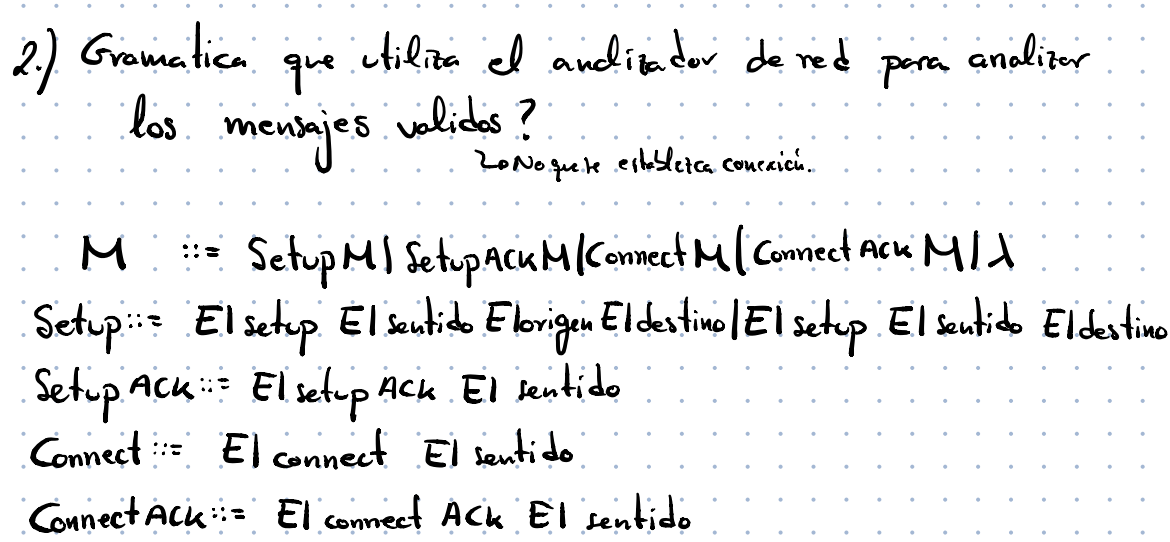
\includegraphics[scale=.3]{image-20210305192731385.png}}
\end{figure}

\chapter{Tema 3: Análisis Sintáctico}


\section{Introducción}

\begin{figure}[H]
	\ffigbox[\FBwidth]
	{\caption{Diagrama Análisis Sintáctico}}
	{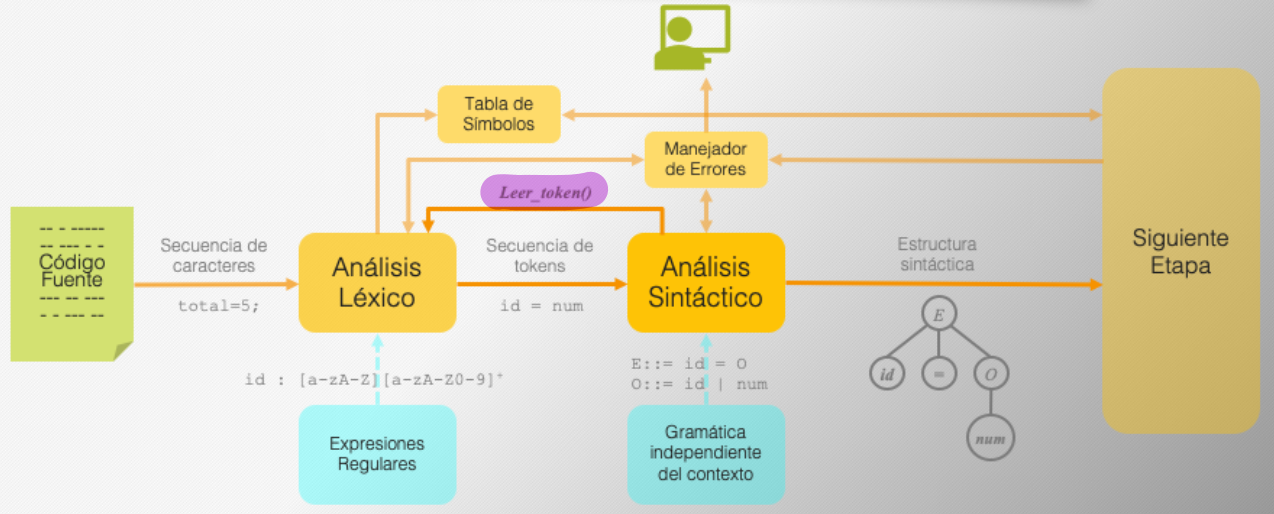
\includegraphics[scale=.3]{image-20210312115053541.png}}
\end{figure}

Su función es comprobar que la secuencia de componentes léxicos es una
secuencia del lenguaje y generar el árbol sintáctico (explicito o no)

Los lenguajes de programación que debe reconocer normalmente son
independientes del contexto, por lo que se representan con gramáticas de
tipo 2, diagramas de sintaxis o autómatas a pila.

\textbf{Ventajas de utilizar gramáticas:}

\begin{itemize}

\item
  Son especificaciones sintácticas y precisas de lenguajes.
\item
  Se puede generar automáticamente un analizador.
\item
  Mientras se construye se pueden descubrir inconsistencias,
  ambigüedades,\ldots{}
\item
  Da estructura al lenguaje de programación lo que hace que sea más
  fácil de generar código y detectar errores.
\item
  Fácil de ampliar y modificar el lenguaje.
\end{itemize}

Nos interesan los analizadores deterministas, que son los que de un
estado con un símbolo solo puede ir a 1 estado. También admitiremos las
transiciones con \(\lambda\).

\textbf{Tipos de analizadores:}

\begin{itemize}
\item \textbf{Descendente}: Va desde la raíz (axioma) hasta las hojas
  (tokens, símbolos terminales. Nosotros trataremos los predictivos
  solo, que son capaces de elegir el token correcto en cada momento, no
  los que tienen retroceso.

  \textbf{LL(k)}, LL(1) Tengo que leer k tokens para identificar que
  regla de producción usar.
\item \textbf{Ascendente}: Va de los nodos hojas(secuencia de tokens) hasta
  la raíz (axioma). Es predictivo.

  \textbf{LR(k)}, que puede ser LR(0), SLR(1), LALR(1) y LR(1)
\end{itemize}

LR significa que lee de izquierda a derecha (LX) y elige la producción
más a la derecha (XR, right).

\section{Análisis Sintáctico Descendiente}

Tenemos una secuencia de tokens x y el objetivo es \textbf{determinar si
la secuencia es una secuencia del lenguaje} definido por la gramática G.
El proceso que seguimos es:

\begin{enumerate}
\def\labelenumi{\arabic{enumi}.}

\item
  \textbf{Partir del axioma} la forma sentencial.
\item
  \textbf{Coger un token de izquierda a derecha.}
\item
  \textbf{Seleccionar una regla de producción}. Se debe sabe
  \textbf{según el token actual} la regla que usar.
\item
  \textbf{Si coinciden} token y símbolo de la forma sentencial, se
  \textbf{lee el siguiente token}.
\item
  \textbf{Sustituir el símbolo no terminal} de la forma sentencial por
  la parte derecha de la regla elegida.
\item
  \textbf{Repetir} el proceso hasta que la entrada haya sido procesada.
\end{enumerate}


\subsection{Con Retroceso}

Lo que cambia es la manera de seleccionar la regla, este \textbf{lo hace
por búsqueda en profundidad con retroceso} lo que hace que tenga una
\textbf{complejidad de \(O(k^n)\)}.


\subsection{Predictivo}

\textbf{Analizador que sólo necesita conocer \(k\) tokens de la cadena
de entrada, para determinar la regla de producción} que debe aplicarse.
El número de tokens, \(k\), necesarios para tomar la decisión de que
regla de producción aplicar, define el nombre del analizador, \(LL(k)\),
\(LR(k)\)

\textbf{Características:}

\begin{itemize}

\item
  Son autómatas a pila deterministas por vaciado.
\item
  No hay retroceso, usa autómatas a pila deterministas predictivos.
\item
  La \textbf{complejidad es líneas} \(O(n)\), tal que n es el número de
  tokens que hay en la sentencia (preferible al exponencial del con
  retroceso)
\end{itemize}

Para evitar problemas a la hora de seleccionar una regla de selección
\textbf{se debe elimina la Recursividad a izquierda y Factorizamos a
izquierdas}. La recursividad a izquierdas hay que evitarla desde el
principio, pero la factorización si se produce no es un gran problema es
fácil de resolverla.

\begin{figure}[H]
	\ffigbox[\FBwidth]
	{\caption{Diagrama Análisis Sintáctico}}
	{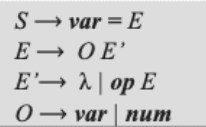
\includegraphics[scale=.4]{image-20210312125711682.png}
	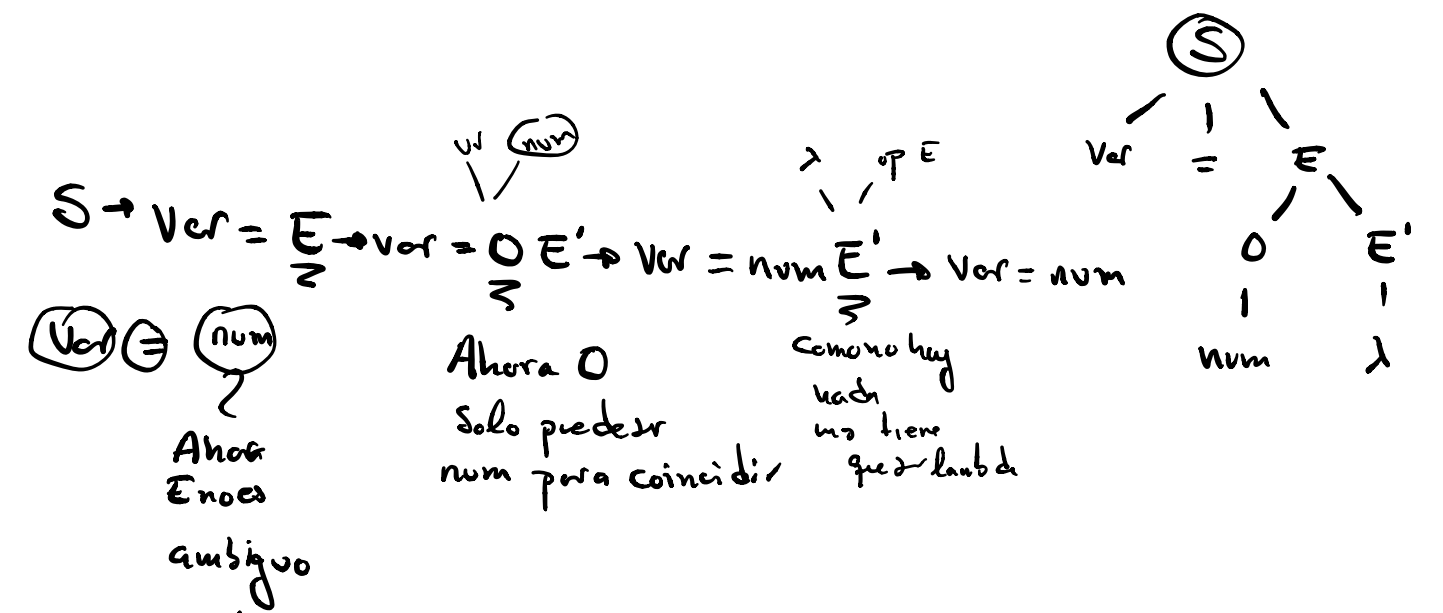
\includegraphics[scale=.2]{image-20210312125654582.png}}
\end{figure}

En los casos que se tienen varias reglas de producción entre las que
elegir usará el conjunto primero del terminar más a la izquierda.


\subsubsection{Conjunto Primero}

\(PRIMERO(\alpha)\) Todos los Terminales que aparecen más a la izquierda
que se derivan de esa forma sentencial. \textbf{Son los posibles
terminales que pueden aparecer más a la izquierda de cualquier secuencia
de producciones de \(\alpha\).} 
\begin{figure}[H]
  $PRIMERO(\alpha)=\{ x | (\alpha \rightarrow _* x \cdot \beta), (x \in \Sigma_T \cup \Sigma^*)\}$

  \captionsetup{justification=centering}
  \caption{Conjunto Primero}
\end{figure}
Si \(X=\lambda \Rightarrow PRIMERO(X)=\{\lambda\}\)

Si \(X \in \Sigma_T \Rightarrow PRIMERO(X)=\{X\}\) El conjunto primero
de un terminal es él mismo.

Si X tiene alguna regla que empieza por un No Terminal es como calcular
el conjunto primero de éste. Ojo con lambda.


\subsubsection{Conjunto Siguiente}

Conjunto primero de todo lo que aparece concatenado de un símbolo No
terminal en todas las formas senténciales que se derivan del axioma. Son
todos los símbolos Terminales que se producen al derivar desde el
axioma.

El conjunto siguiente nunca va a contener a \(\lambda\). \$ es el token
que indica fin de sentencia.

Se aplica sobre los No Terminales de la parte de la derecha de todas las
producciones. 
\begin{figure}[H]
  $SIGUIENTE(A)=\{ x | (S \rightarrow _*\alpha A \beta), (A \in \Sigma_N), (\alpha \in \Sigma^*), (\beta \in \Sigma^+),(x\in PRIMERO(\beta)-\{\lambda\})\}$

  \captionsetup{justification=centering}
  \caption{Conjunto Siguiente}
\end{figure}
Fases:

\begin{itemize}

\item
  Obtener las reglas de formación de los conjuntos siguientes. Se aplica
  sobre todos los NT de la derecha de la regla de producción. Tiene la
  forma de \(A \rightarrow \alpha B \beta\), se asocian las partes de la
  regla con los símbolos, donde B es el NT sobre del que queremos el
  S(B).

\begin{enumerate}
\def\labelenumi{\arabic{enumi}.}
\item
  El conjunto siguiente del axioma es \$ siempre, pero hay que aplicar
  el conjunto siguiente sobre sus reglas.
\item
  Se aplica \(S(B)=S(B)\cup PRIMERO(\beta)-\{\lambda\}\), que si no hay
  \(\beta\) hace que esta regla no haga nada y se haga la siguiente.
\item
  Si \(PRIMERO(\beta)\) contiene a \(\lambda\) también se aplica,
  \(S(B)=S(B)\cup S(A)\)
\end{enumerate}


\item
  Ir aplicando las reglas, escribiendo los T en una tabla, hasta que el
  conjunto siguiente no cambie en una iteración.
\end{itemize}

\subsubsection{Conjunto de Predicción}

Es el criterio para determinar que regla expandir para un símbolo no
terminal, y se aplica sobre las reglas de producción completa.

Dado \(A \rightarrow \alpha\):

\begin{figure}[H]
 \begin{eqnarray*}
    PREDICCION(A \rightarrow \alpha) &=& PRIMERO(\alpha) / \lambda \notin PRIMERO(\alpha) \\
    PREDICCION(A \rightarrow \alpha) &=& [PRIMERO(\alpha)-\{\lambda\}] \cup S(A) / \lambda \in PRIMERO(\alpha)
 \end{eqnarray*}

  \captionsetup{justification=centering}
  \caption{Conjunto de Predicción}
\end{figure}

\pagebreak
\subsubsection{Condiciones LL}

Condiciones que debe tener para hacer Análisis Sintáctico Descendente
Predictivo.
Estas condiciones se aplican sobre NT que tienen más de una regla de
producción.

\begin{enumerate}
\def\labelenumi{\arabic{enumi}.}

\item
  \textbf{Condición PRIMERO-PRIMERO:} Los conjuntos primeros de las
  reglas de producción del NT deben ser disjuntos (no tengas símbolos en
  común).

  \(A \rightarrow \alpha_1 |...|\alpha_n, P(\alpha_1) \cap ... \cap P(\alpha_n) = \empty\)
\item
  \textbf{Condición PRIMERO-SIGUIENTE}: Esta se aplica cuando alguna de
  las reglas tienen en su conjunto primero \(\lambda\), entonces el
  conjunto primero del resto de las reglas (sin incluir la de lambda)
  deben ser disjuntas con el conjunto siguiente del NT de la izquierda.
\end{enumerate}


\subsubsection{Análisis Descendente Recursivo}


\paragraph{Estrategia}

Para construirlo se crea un procedimiento por cada NT que sea capaz de
reconocer las distintas reglas de producción que tiene asociadas, para
ello va leyendo símbolo a símbolo con token\_actual, siguiendo las
siguientes reglas:

\begin{itemize}

\item
  Si se lee un Terminal: Si coincide el token\_actual con lo esperado
  lee el siguiente token, sino coincide da error sintáctico.
\item
  Si se lee un NT: Se llama al procedimiento del NT que se encargara de
  reconocerlo.
\item
  Si se lee una lambda: No se hace nada.
\end{itemize}

Si la pila se vacía y la entrada ha sido procesada entonces la secuencia
de tokens es reconocida, entonces iría al analizador semántico.


\paragraph{Ventajas}

\begin{itemize}

\item
  Requieren formalizar una gramática.
\item
  Son fáciles de escribir e interpretar.
\item
  Adecuados para analizadores simples.
\end{itemize}


\paragraph{Inconvenientes}

\begin{itemize}

\item
  Difíciles de ampliar y mantener.
\item
  Coste computacional asociado a la recursividad.
\item
  Construcción específica para el lenguaje reconocido.
\item
  Conjunto reducido de lenguajes independientes de contexto.
\end{itemize}
 
\pagebreak

\subsubsection{Ejemplo:}

\begin{figure}[H]
	\ffigbox[\FBwidth]
	{\caption{Descendente Recursivo: Gramática y Procedimiento Axioma}}
	{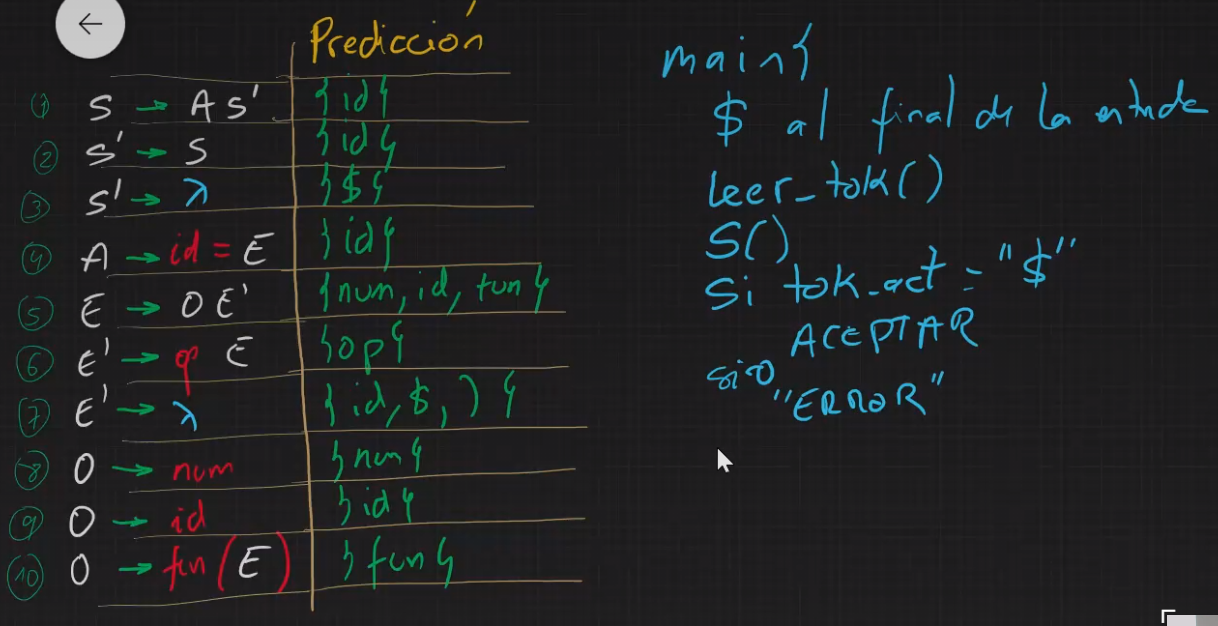
\includegraphics[scale=.4]{2021-03-26 17_49_53-Ejercicio descendente recursivo.png}}
\end{figure}

\begin{figure}[H]
	\ffigbox[\FBwidth]
	{\caption{Descendente Recursivo: Procedimientos}}
	{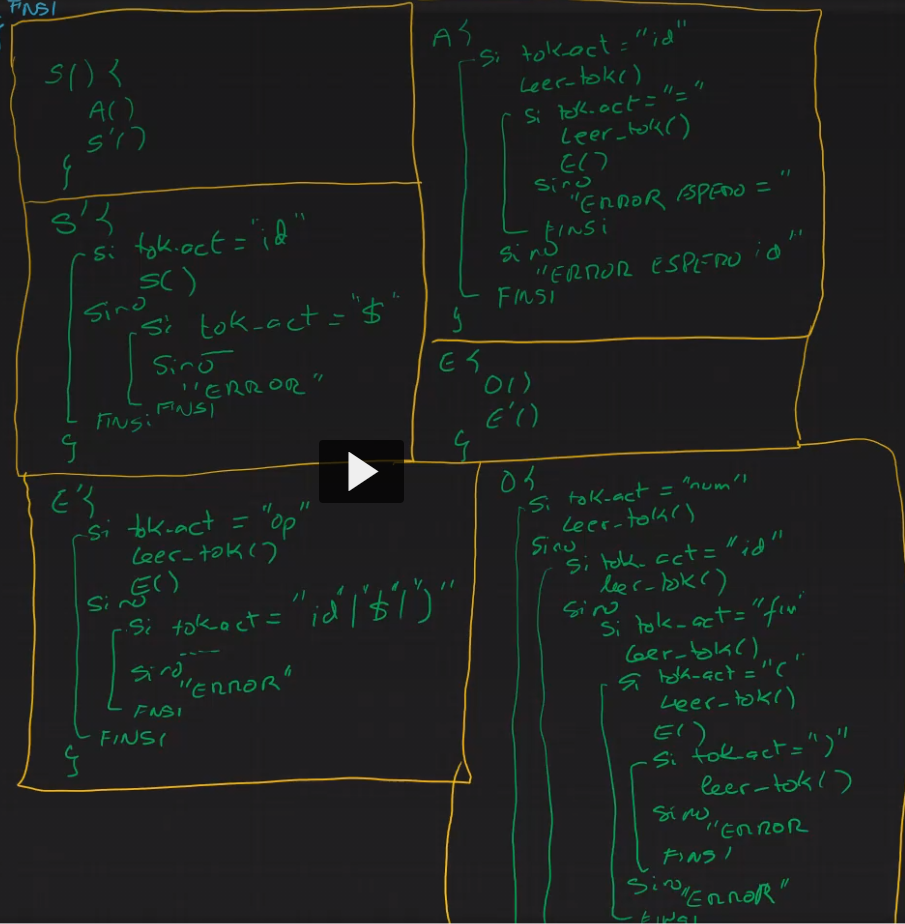
\includegraphics[scale=.5]{Untitled 102.png}}
\end{figure}

\begin{figure}[H]
	\ffigbox[\FBwidth]
	{\caption{Descendente Recursivo: Reconocimiento secuencia}}
	{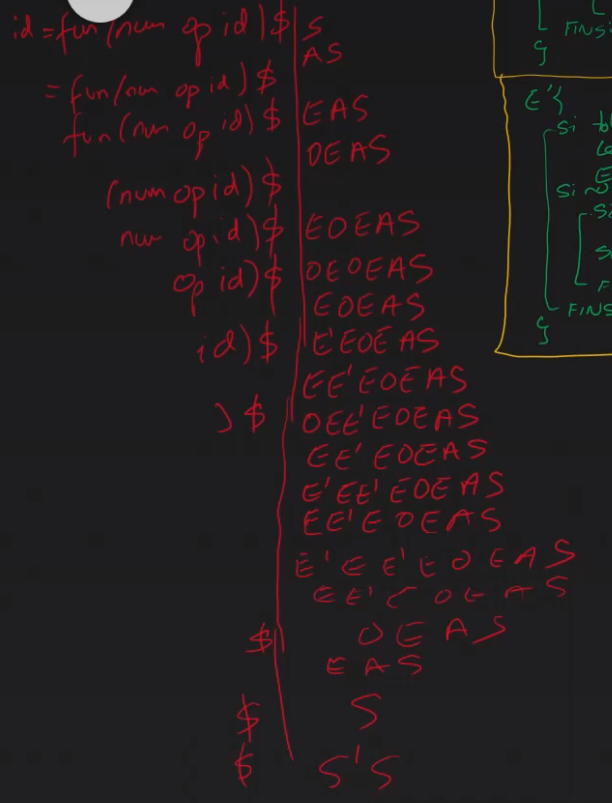
\includegraphics[scale=.7]{2021-03-26 17_50_51-Ejercicio descendente recursivo.png}}
\end{figure}

\pagebreak

\subsubsection{Análisis Sintáctico LL(1)}

Es un analizador predictivo que procesa los tokens de izquierda a
derecha, con derivaciones más a la izquierda.

Necesita sólo 1 símbolo de preanálisis para determinar qué producción
aplicar.


\subsubsection{Análisis Descendente Dirigido por tablas}

Características:

\begin{itemize}

\item
  Se construye en árbol de derivación desde el axioma.
\item
  La cima de la pila determina la operación a realizar.
\item
  La sustitución de los símbolos no terminales por producciones está
  definida en una tabla, en la que las filas son los NT y las columnas
  los T.
\item
  Debe cumplir las condiciones LL para analizarse con LL(1)
\end{itemize}

Construcción de la tabla: Se construye con el Conjunto de Predicción,
filas NT y columnas Terminales y \$.

\begin{itemize}

\item
  Dentro se ponen las reglas de producción, que se ponen en la fila del
  NT de la izquierda de la regla y en las columnas de todos los T del
  conjunto de predicción de la regla.
\end{itemize}

La idea general es:

\begin{itemize}

\item
  Si el símbolo de preanálisis y la cima de la pila son \$ es que hemos
  terminado con éxito.
\item
  Si el símbolo de preanálisis en es un T y la cima de pila es el mismo,
  pero no \$ (seria final), se saca de la pila y se lee token (lo que lo
  saca de la secuencia a reconocer)
\item
  Si el símbolo de cima de pila es un NT, se consulta la fila del NT y
  la columna del símbolo de preanálisis, si esta está vacía error sino
  se meta en la cima de la pila.
\end{itemize}

\pagebreak

\subsubsection{Ejemplo completo}

\begin{enumerate}
\def\labelenumi{\arabic{enumi}.}

\item
  Calcular Conjuntos Primeros.
\item
  Calcular Conjuntos Siguientes.
\item
  Calcular Conjuntos de Predicción.

\begin{figure}[H]
	\ffigbox[\FBwidth]
	{\caption{Calculo de Conj. Primero, Siguiente y Predicción}}
	{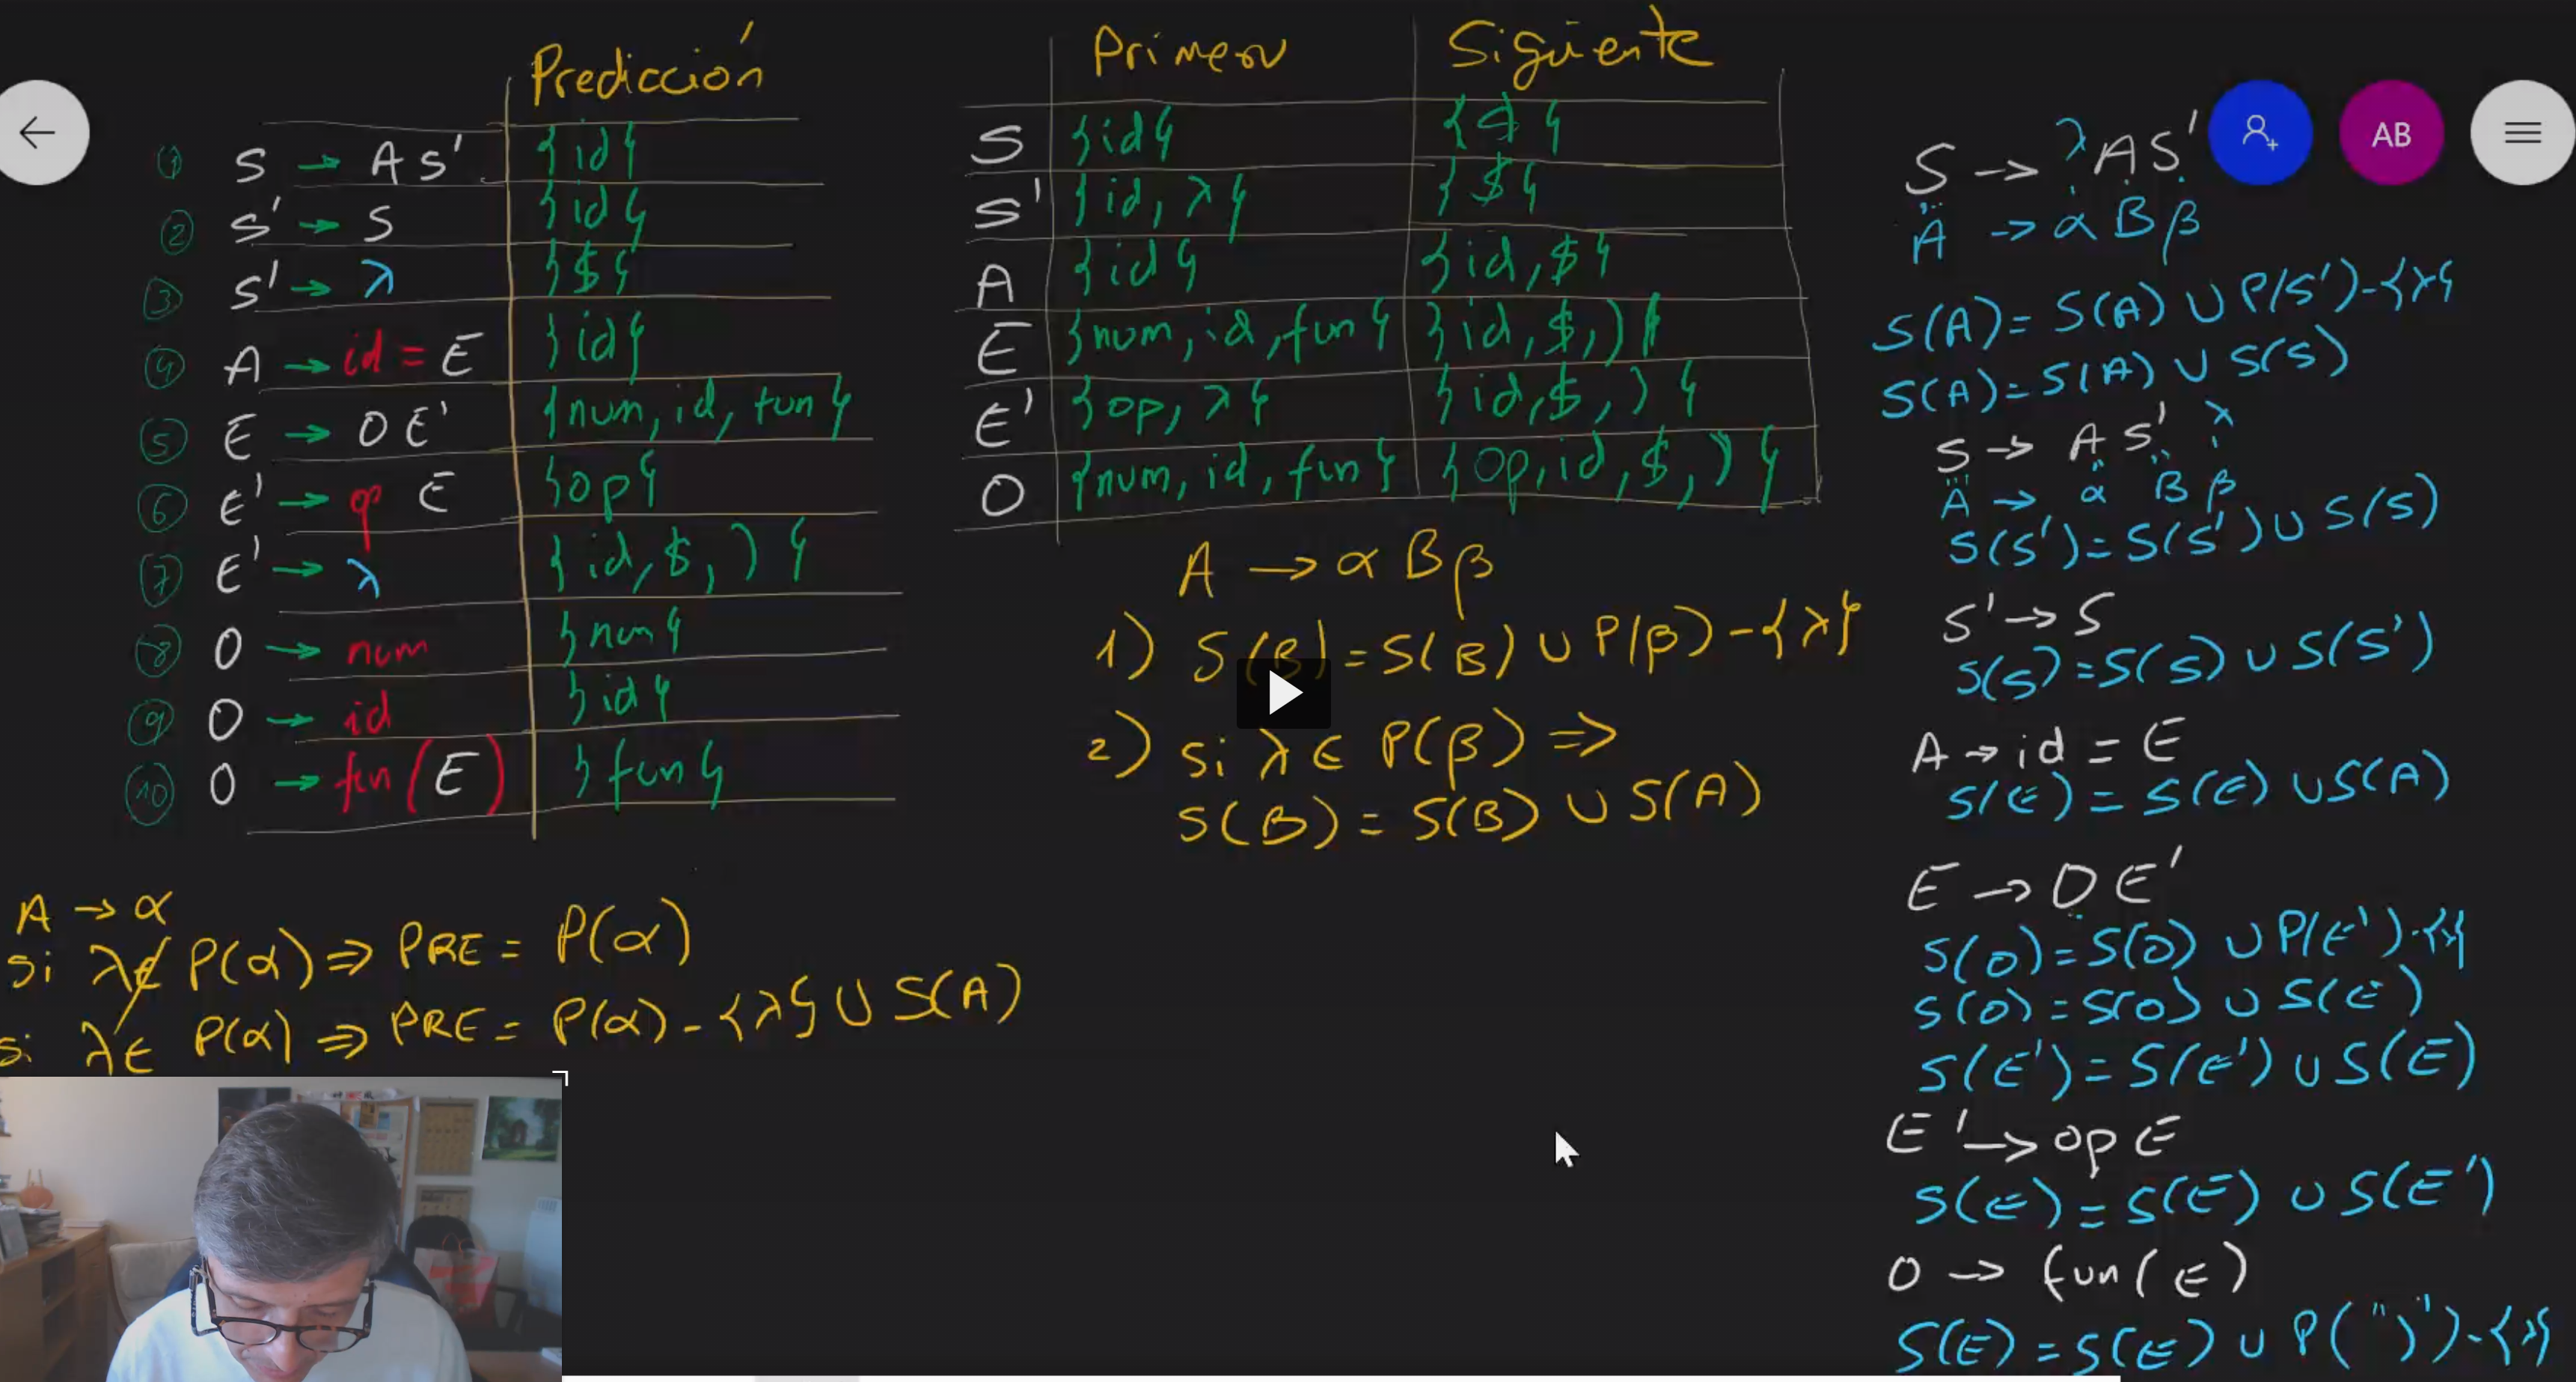
\includegraphics[scale=.12]{image-20210320110844879.png}}
\end{figure}

\item
  Comprobación de la Condiciones de
  LL(1)
  
  \begin{figure}[H]
	\ffigbox[\FBwidth]
	{\caption{Comprobación de Condiciones LL(1)}}
	{\includegraphics[scale=.17]{image-20210320110940170.png}}
\end{figure}

\pagebreak
\item
  Tabla de Conjuntos de Predicción


  \begin{figure}[H]
	\ffigbox[\FBwidth]
	{\caption{Construcción de Tabla de Conjuntos de Predicción}}
	{\includegraphics[scale=.2]{image-20210320111419566.png}}
\end{figure}

\item
  Prueba de lectura de secuencia de entrada (falta que se vaya ) y los
  NT que quedan se van con el \$)

\begin{figure}[H]
	\ffigbox[\FBwidth]
	{\caption{Prueba de lectura de secuencias ASI}}
	{\includegraphics[scale=.23]{image-20210320111752355.png}}
\end{figure}
  
\end{enumerate}

\section{Análisis Sintáctico Ascendente}

Una secuencia de tokens x pertenece al lenguaje definido por G si genera una secuencia valida del lenguaje. Se van aplicando reglas de producción que generan un árbol sintáctico.

\begin{enumerate}
  \item Coger tokens de izquierda a derecha.
  \item Buscar el pivote de reducción (que reduciremos)
  \item Aplicar derivaciones más a la derecha, sustituyen por NT.
  \item Repetir el proceso hasta que la entrada ha sido procesada y reducida al axioma.
\end{enumerate}

\textbf{Pivote de reducción:} Subcadena w de una forma sentencial x, $x \in \sum^+$, que es la parte derecha de una regla de producción y sustituye a la inversa, mete el NT del lado izquierdo. 

La decisión es si añadir otro terminal al pivote (desplazar) o aplicar la producción en orden inverso.
\begin{itemize}
  \item $x=uwv, A \rightarrow w | S \rightarrow uAv$
  \item Reduce el pivote más a la izquierda.
  \item A la derecha del pivote solo hay terminales o $\lambda$.
  \item El pivote se puede buscar utilizando una pila.
\end{itemize}

\subsection{Prefijo} 
Terminales y No Terminales que se pueden encontrar en pila, que nos permite llegar al axioma.

\subsection{Prefijo viable} 
Terminales y No Terminales que pueden encontrarse en la pila y pueden formar parte de un pivote que permita reducir hasta el axioma. 

Un prefijo de un prefijo viable también es un prefijo viable.

La estrategia es construir un autómata que reconozca los prefijos viables de la gramática, el autómata LR(0) los reconoce.

\begin{figure}[H]
	\ffigbox[\FBwidth]
	{\caption{Prefijos viables}}
	{\includegraphics[scale=.4]{2021-03-26 18_27_20-ASintactico.pdf - Foxit Reader.png}}
\end{figure}
  
\subsection{Análisis LR}
Para algunas gramáticas independientes de contexto, LR(k), se puede construir un autómata a pila determinista.

\begin{itemize}
  \item k es la cantidad de símbolos de preanálisis necesarios para tomas una decisión.
\end{itemize}

Tipos de analizadores:
\begin{itemize}
  \item \textbf{SLR(1)} es un LR simple. La clase más pequeña de gramáticas, numero de estados más pequeño, simple y rápida.
  \item \textbf{LR(1)}. La clase más grande de gramáticas, el mayor número de estados, construcción larga y penosa.
  \item \textbf{LALR(1)}. La clase intermedia de gramáticas, numero de estados como SLR(1), construcción larga y penosa.
\end{itemize}
En cuanto a que gramáticas pueden representas: $G2>LR>LALR>SLR$

\begin{figure}[H]
	\ffigbox[\FBwidth]
	{\caption{Comparación de grámaticas}}
	{\includegraphics[scale=.57]{2021-04-13 15_35_24-ASintactico.pdf - Foxit Reader.png}}
\end{figure}

\subsection{Análisis Sintáctico LR(1)}

\subsubsection{Esquema del Análisis Ascendente dirigido por tabla}
En este caso las filas son el Conjunto LR(0), también llamado \textbf{conjunto LR canónico}, que son todos los estados resultados de hacer el cierre del axioma y los sucesivos Ir$\_$a.

Las columnas son \textbf{Acciones}, Terminales y \$, y por otro lado \textbf{Ir$\_$a}, No Terminales.

\subsubsection{Item LR(0)}

Son reglas de producción con $\cdot$, que indica que lo de la izquierda está en la pila.
\begin{itemize}
  \item $A \rightarrow \alpha \beta \cdot \gamma$, $\alpha,\beta$ en pila.
  \item Los símbolos a la derecha todavía no se han procesado. $\gamma$ sin procesar.
  \item Cuando se produce que a la derecha de $\cdot$ no hay símbolos es posible que haya encontrado un pivote de reducción.
\end{itemize}

\pagebreak

\subsubsection{Analizador LR(0)}
A partir de los ítems se puede construir un AFD que realice el análisis de prefijos viables.

Los estados de ese AFD se les llama \textbf{Conjunto canónico LR(0)}, que es lo que buscamos para la tabla, cada uno de esos estados está formado por un conjunto de ítems.

Cuando el axioma tenga varias producciones, se amplía la gramática, haciendo que un nuevo NT sea el axioma y produzca el axioma anterior. $S'\rightarrow S$

\textbf{Para crear los estados del Conjunto canónico LR(0) utilizaremos:}
\begin{itemize}
  \item \textbf{Cierre(ítems)} Determina los ítems que pertenecen a un estado. 
  
  Lo que hace es añadir a todas las reglas de producción del NT izquierdo, el punto $\cdot$ a la izquierda. Además, si el punto está justo a la izquierda de un NT se hace también para sus reglas. 
  \begin{figure}[H]
    \ffigbox[\FBwidth]
    {\caption{Cierre(ítems)}}
    {\includegraphics[scale=.4]{2021-03-26 19_10_20-ASintactico.pdf - Foxit Reader.png}}
  \end{figure}
  
  \item \textbf{Ir$\_$a(ítems, Símbolo)} Genera un nuevo estado a partir de los ítems de un estado y símbolo gramaticales.
  
  Hace el cierre de pasar el punto al otro lado de Símbolo, que se pasa como parámetro. Es vacío cuando no hay ningún item que tenga el punto a su izquierda.
  \begin{figure}[H]
    \ffigbox[\FBwidth]
    {\caption{Ir$\_$a(ítems, Símbolo)}}
    {\includegraphics[scale=.4]{2021-03-26 19_14_19-ASintactico.pdf - Foxit Reader.png}}
  \end{figure}
\end{itemize}

El analizador LR(0) es un Autómata con Pila Determinista, los estados del analizador son conjuntos de ítems.

\textbf{Algoritmo de creación del analizador LR(0)}
\begin{enumerate}
  \item Crear el conjunto canónico LR(0)
  \begin{enumerate}
    \item Ampliar la gramática $S'\rightarrow S$, cuando axioma tiene más de una regla.
    \item $E_0 = Cierre(S'\rightarrow S)$.
    \item Repetir mientras son creados nuevos estados, $E_i = Ir\_a(I_k, \alpha), \forall \alpha \in \sum^+$, hacer para aquellos símbolos que estén a la derecha de un punto, si no darán vacío y no nos son de utilidad. Que crea tantos estados como posibles aplicaciones de la función Ir$\_$a en todos los estados, mientras no genere estados exactamente iguales, pero puede haber reglas repetidas.
  \end{enumerate}
  \item Asociar acciones a los ítems de los estados, que son: Desplazar, Reducir, Ir a otro estado, Aceptar y Error.
\end{enumerate}

Ejemplo: 
\begin{figure}[H]
  \ffigbox[\FBwidth]
  {\caption{Generar Conjunto Canónico LR(0)}}
  {\includegraphics[scale=.3]{2021-03-26 19_23_58-ASintactico.pdf - Foxit Reader.png}}
\end{figure}
\pagebreak
\textbf{Asociar acciones a los ítems de los estados:}
\begin{itemize}
  \item $\forall I_k = \{ A \rightarrow \alpha \cdot x \beta\} I_k \in E_j \space y \space x\in \sum_T, Accion(E_j, x)=Desplazar E_n, E_n = Ir\_a(E_j,x)$
  \item $\forall I_k = \{ A \rightarrow \alpha \cdot X \beta\} I_k \in E_j \space y \space X\in \sum_N, Ir\_a(E_j,X) = E_n$
  \item $\forall I_k = \{ A \rightarrow \alpha \cdot \} I_k \in E_j, Accion(E_j, x)= Reducir A \rightarrow \alpha, \forall x \in \{ \sum_T, \$ \}$
  \item $I_k = \{ S' \rightarrow S \cdot \} I_k \in E_j, Accion(E_j, \$)= Aceptar$
\end{itemize}

Ejemplo: 
\begin{figure}[H]
  \ffigbox[\FBwidth]
  {\caption{Analizador LR(0)}}
  {\includegraphics[scale=.35]{2021-03-26 19_51_21-ASintactico.pdf - Foxit Reader.png}}
\end{figure}

LR(0) toma la decisión de desplazar o reducir SIN depender del token de entrada, solo del estado, pero si del estado al que transita.

Se puede producir \textbf{Conflicto de Reducción-Desplazamiento}, cuando para un mismo estado y símbolo hay dos acciones.
Para solventar esto se amplía el LR(0) a SLR(1)

\textbf{Ventajas}
\begin{itemize}
  \item Fáciles de construir.
  \item Las reducciones están asociadas a estados.
\end{itemize}

\textbf{Inconvenientes}
\begin{enumerate}
  \item Son muy pocas las que se pueden utilizar.
  \item Estrategias de recuperación de error.
\end{enumerate}

\subsection{Análisis SLR(1)}
Es un Autómata con Pila Determinista.
\begin{itemize}
  \item Los estados del analizador son conjuntos de ítems.
\end{itemize}

Se construye igual que el analizar LR(0), pero la asignación de la acción Reducir cambia.

\textbf{Algoritmo de creación del analizador SLR(1)}
\begin{itemize}
  \item Crear el conjunto canónico LR(0), los estados.
  \item Asociar acciones (Desplazar, Reducir, Ir\_a, Aceptar, Error) a los ítems de los estados.
\end{itemize}

\textbf{Asociar acciones a los ítems de los estados:}
\begin{itemize}
  \item $\forall I_k = \{ A \rightarrow \alpha \cdot x \beta\} I_k \in E_j \space y \space x\in \sum_T, Accion(E_j, x)=Desplazar E_n, E_n = Ir\_a(E_j,x)$
  \item $\forall I_k = \{ A \rightarrow \alpha \cdot X \beta\} I_k \in E_j \space y \space X\in \sum_N, Ir\_a(E_j,X) = E_n$
  \item $\forall I_k = \{ A \rightarrow \alpha \cdot \} I_k \in E_j, Accion(E_j, x)= Reducir A \rightarrow \alpha, \forall x \in Siguiente(A), \alpha \in \sum ^*$ Se pone reducción solo para los T de $S(A)$
  \item $I_k = \{ S' \rightarrow S \cdot \} I_k \in E_j, Accion(E_j, \$)= Aceptar$
\end{itemize}

Cuando se indica R2, indica que la regla que se reduce es la numerada como 2.

\textbf{Condiciones SLR(1):}
Tienen que cumplirse dos condiciones para poder hace un análisis SLR(1). 

No es necesario eliminar la recursividad a derechas e izquierda y ni es necesario factorizar.

\begin{itemize}
  \item Sin conflictos \textbf{Desplazamiento-Reducción}, debe darse que en los estados que haya reducciones no haya otro item que tenga desplazar para un símbolo del conjunto siguiente de la reducción.
  
  $A \rightarrow \alpha \cdot x \beta$

  $B \rightarrow \alpha \cdot$

  Entonces $x \notin Siguiente(B)$

  \item Sin conflictos \textbf{Reducción-Reducción}, debe cumplir que cuando haya más de una regla de reducción en un estado, sus conjuntos siguientes sean disjuntos.
    
  $A \rightarrow \alpha \cdot $

  $B \rightarrow \gamma \cdot$

  Entonces $Siguiente(A) \cap Siguiente(B)$
\end{itemize}

\includepdf[pages=78]{docs/ASintactico.pdf}

\begin{figure}[H]
  \ffigbox[\FBwidth]
  {\caption{Ejemplo analizador SLR(1)}}
  {\includegraphics[scale=.5]{2021-04-13 14_59_35-ASintactico.pdf - Foxit Reader.png}}
\end{figure}

\subsection{Comparación LL vs LR}
\textbf{Simplicidad:} LL es más fácil de construir y completar.

\textbf{Tamaño:} LL es más pequeño.

\textbf{Generalidad:} Todas las LL son LR, pero no al contrario.

\textbf{Detección de error:} LR requiere menos acciones para detectar el error.

\textbf{Recuperación de errores:} LL es más sencillo de implementar.

\chapter{Tema 4: Análisis Semántico}

\section{Introducción}
El análisis semántico es una \textbf{extensión del análisis sintáctico para la compresión del programa}, para comprobar que tiene sentido y que está conectado. Destaca por la verificación de tipos.

Es un paso \textbf{previo a su traducción, aunque hay partes que se pueden ir haciendo}. También modifica la tabla de símbolos.

Las gramáticas independientes del contexto \textbf{(G2) no son suficientes para este análisis}, se necesita realizar comprobaciones de larga distancia en el árbol sintáctico (que no se pueden representar con reglas de producción) y no solo comprobar que se deriva de la gramática del lenguaje.

Para cumplir lo anterior se utilizan Gramáticas de atributos (gramáticas atribuidas), que son más ricas.

\textbf{ Algunas de las comprobaciones que se realizan durante el Análisis Semántico:}
\begin{itemize}
  \item Comprobación de \textbf{tipos}, los operadores y operandos deben ser compatibles.
  \item Comprobaciones de \textbf{unicidad}, en aquellas situaciones en los que un objetico solo puede definirse una vez exclusivamente.
  \item Comprobaciones \textbf{relacionadas con nombres}, cuando el mismo nombre debe aparecer dos o más veces.
  \item Comprobación del \textbf{flujo de control}, controlar las proposiciones para abandonar el flujo de control, que tiene finalización.
\end{itemize}
\pagebreak
\section{Gramáticas atribuidas}
Son gramáticas G2 a las que se añaden atributos y reglas de evaluación de atributos (reglas semánticas).
\begin{itemize}
  \item Cada \textbf{atributo} es una variable que representa una propiedad del símbolo terminal o no terminal, puede ser una cadena , numero, tipo, posición de memoria, etc.
  \item \textbf{Reglas semánticas} (Reglas para calcular/Reglas para comprobar), se asocian a las producciones sintácticas (reglas de producción). Se definen en función de los atributos de los símbolos en la producción.
  \item Sobre los atributos y reglas hay unas condiciones semánticas.
\end{itemize}

Se pueden construir Arboles adornador o decorados, donde se muestra la relación entre atributos de una misma regla de producción.

\textbf{Gramáticas atribuida $GA=\{G,A,R,B\}$}
\begin{itemize}
  \item G - \textbf{Gramática} libre de contexto (G2), $G = \{\Sigma_N, \Sigma_T, S, P\}$.
  \item A - Conjunto de \textbf{atributos} asociados a cada símbolo X. Son disjuntos.
  \item R - \textbf{Reglas semánticas} asociadas a cada regla en P.
  \item B - \textbf{Condiciones} asociadas a cada regla de P.
\end{itemize}

\textbf{Existen diferentes Especificaciones:}
\begin{itemize}
  \item \textbf{DDS - Definición dirigida por la sintaxis}, acciones tras cada producción (sin orden específicos).
  
  \begin{figure}[H]
    \ffigbox[\FBwidth]
    {\caption{Ejemplo DDS}}
    {\includegraphics[scale=.3]{2021-04-21 10_49_57-05_resum_Sem_2021.pdf - Foxit Reader.png}}
  \end{figure}

  \item \textbf{EDT - Esquema de Traducción}, las acciones semánticas se intercalan con los símbolos de la producción, indicando el orden de ejecución de las acciones semánticas. Es una notación para hacer un traductor. Tiene dos tipos:
  \begin{itemize}
    \item EDT \textbf{solo con atributos sintetizados}, las acciones se ponen al final de la producción.
    \item EDT con \textbf{atributos sintetizados y heredados}, la posición de las acciones debe tener en cuenta los cálculos y atributos que contribuyen.
    \begin{itemize}
      \item Un atributo heredado (en la parte derecha de la producción) DEBE calculará con una acción antes de dicho símbolo.
      \item Una acción NO debe referirse a un atributo sintetizado de un símbolo que este la derecha de la acción.
      \item Para calcular el No Terminal izquierdo DEBE haberse calculado previamente todos los atributos de los símbolos que participen.
    \end{itemize}
  \end{itemize}
  \begin{figure}[H]
    \ffigbox[\FBwidth]
    {\caption{Ejemplo DDS}}
    {\includegraphics[scale=.3]{2021-04-21 11_14_06-05_resum_Sem_2021.pdf - Foxit Reader.png}
    \includegraphics[scale=.24]{2021-04-21 11_14_40-05_resum_Sem_2021.pdf - Foxit Reader.png}}
  \end{figure}
\end{itemize}

Una gramática atribuida GA es \textbf{completa} si, para todo atributo de toda regla hay una acción semántica asociada para calcularlo.
\begin{itemize}
  \item Para toda regla P: $X\rightarrow\alpha$ en P, AS(X) está en AC(P).
  \item Para toda regla Q: $Y\rightarrow\alpha X \beta$ en Q, AH(X) está en AC(Q).
  \item $AS(X) \cup AH(X) = A(X)$ $AS(X) \cap AH(X)=\emptyset$
\end{itemize}

Una gramática atribuida GA esta \textbf{bien definida} si, para cualquier sentencia en L(GA), todos los atributos pueden ser calculados (este proceso se llama evaluación de la gramática). Además, una sentencia de su lenguaje tiene atributos correctos si se verifican las condiciones en B(P) para cada regla P de la gramática.
\begin{itemize}
  \item \textbf{Gramática Atribuida bien definida $\Rightarrow$ Gramática Atribuida completa}
\end{itemize}
En el caso de buscar que este bien definida es más fácil buscar un fallo (para decir que no lo es), que comprobar que se cumple para todas las sentencias del lenguaje (que es inabarcable). Si no se encuentra el contraejemplo se dice que no se puede demostrar que no lo es.

\section{Tipos de atributos y gramáticas}
\subsection{Atributos heredados y sintetizados}
\textbf{Dos tipos de atributos:}
\begin{itemize}
  \item \textbf{Sintetizados:} El valor de un nodo (parte izquierda) depende solo de los valores de los nodos hijos (parte derecha). Se hace de abajo hacia arriba.
  \begin{figure}[H]
    \ffigbox[\FBwidth]
    {\caption{A. sintetizado}}
    {\includegraphics[scale=.3]{2021-04-21 10_46_33-05_resum_Sem_2021.pdf - Foxit Reader.png}}
  \end{figure}

  \item \textbf{Heredados:} Los valores se pasan a niveles inferiores del árbol, el valor depende de los hermanos y del padre (como un sumidero de datos).
  
  \begin{figure}[H]
    \ffigbox[\FBwidth]
    {\caption{A. heredado}}
    {\includegraphics[scale=.3]{2021-04-21 10_47_58-05_resum_Sem_2021.pdf - Foxit Reader.png}}
  \end{figure}

\end{itemize}
Los atributos mantienen su tipo en toda la gramática, y los tokens (símbolos terminales) solo tienen atributos sintetizados.

Los atributos heredados se tratan utilizando estructuras auxiliares para pasar los datos, como puede ser una tabla o una pila.

\textbf{Atributos calculados AC(P):} Atributos calculados con producción P, que exista una regla de cálculo asociada a la obtención de su valor.
\begin{itemize}
  \item \textbf{Atributos sintetizados AS(X):} Cuando lo que se calcula es el símbolo de la parte izquierda de la regla.
  \item \textbf{Atributos heredados AH(X):} Cuando el valor que se calcula es el producido en una regla de producción.
\end{itemize}
\pagebreak
\subsection{Evaluación de las reglas semánticas}
\textbf{Hay dos métodos:}
\begin{itemize}
  \item Métodos con \textbf{árbol de análisis sintáctico}: Se realizan en el momento de compilación y el orden que se sigue viene dado por el grafo de dependencias (ordenamiento topológico) de cada nodo construido según el árbol de análisis sintáctico. No funciona para gramáticas con ciclos.
  \item Métodos de evaluación \textbf{durante el análisis sintáctico}: La evaluación se hace en una sola pasada y no es necesario construir un grafo de dependencias de forma explicita, lo que lo hace más eficiente. 
  \begin{itemize}
    \item Hay métodos \textbf{basados en reglas}, en el que las acciones semánticas asociadas a las producciones se analizan a mano o con alguna herramienta.
    \item Hay métodos \textbf{sin recuerdo}, el orden de evaluación no tiene en cuenta las reglas semánticas.
  \end{itemize}
\end{itemize}

\subsection{Evaluación durante el análisis sintáctico}
\begin{itemize}
  \item \textbf{S-A Grammars - Gramáticas de Atributos Sintetizados:} Gramática donde solo existen atributos sintetizados.
  
  Se puede evaluar con un analizador descendente, mediante una pila, y descendente por medio de rutinas y valores devueltos.
  \item \textbf{L-A Grammars - Gramáticas de Atributos por la Izquierda:} Gramática donde todos los atributos heredados de cualquier producción dependen solo de atributos de símbolos a su izquierda o del símbolo de la parte izquierda de la producción.
  
  La información debe fluir de izquierda a derecha.

  Las L-A de tipo LL(1) pueden evaluarse con analizadores descendentes y ascendentes.

  Solo algunas de las LR(1) que NO son LL(1) pueden evaluarse con L-A mediante un analizador ascendente.
\end{itemize}
\section{Evaluación de atributos}
\subsection{Árbol de dependencia}
\subsection{DDS y TDS}
\section{Árbol de Sintaxis abstracta}
\subsection{Evaluación de varias pasadas}



\end{document}

